\documentclass[11pt,a4paper]{article}
\usepackage[a4paper,margin=2.3cm]{geometry}
\usepackage{amsmath,amssymb,mathtools,amsthm}
\usepackage{fontspec}
\usepackage{polyglossia}
\setmainlanguage{english}
\setotherlanguage{russian}
\setmainfont{Liberation Serif}
\setsansfont{Liberation Sans}
\setmonofont{Liberation Mono}
\newfontfamily\cyrillicfont[Ligatures=TeX]{Liberation Serif}
\newfontfamily\cyrillicfontsf[Ligatures=TeX]{Liberation Sans}
\newfontfamily\cyrillicfonttt{Liberation Mono}
\usepackage{booktabs}
\usepackage{array}
\usepackage{enumitem}
\usepackage{graphicx}
\usepackage{float}
\usepackage{listings}
\usepackage{xcolor}
\usepackage[hidelinks]{hyperref}

\setlength{\parindent}{0pt}
\setlength{\parskip}{0.55em}
\emergencystretch=1.5em
\setlist{itemsep=0.25em,topsep=0.3em}
\setcounter{tocdepth}{2}
\lstset{basicstyle=\ttfamily\footnotesize,columns=fullflexible,keepspaces=true,
  frame=single,rulecolor=\color{black!25},breaklines=true,
  commentstyle=\color{black!55},showstringspaces=false}

\newcommand{\G}{\mathcal{G}_k}
\newcommand{\norm}[1]{\lVert #1\rVert_2}
\newcommand{\E}{\mathbb{E}}
\DeclareMathOperator*{\argmin}{arg\,min}
\DeclareMathOperator{\diag}{diag}
\DeclareMathOperator{\Var}{Var}
\DeclareMathOperator{\sigm}{sigm}
\makeatletter\newcommand{\tabinput}[1]{\@@input #1 }\makeatother


\title{SGD versus Robust SGD under Gradient Uncertainty\\[0.3em]
\large Homework mini-project report}
\author{Egor Chulkov, Vladislav Dvornikov, Daria Demeshko\\[0.2em]\small Optimisation methods for artificial intelligence}
\date{17 November 2026}

\begin{document}
\maketitle

\begin{abstract}
\noindent Robust SGD (R-SGD) chooses each step against the worst gradient in an ellipsoid
$\G$ built from the mini-batch observations. This report derives the robust step, implements it
with an exact $O(p)$ solver, and compares SGD and R-SGD on logistic regression and a two-layer
$\tanh$ network under injected gradient noise.

\emph{Theory.}
\begin{itemize}
\item The step is unique and is never longer than the SGD step.
\item It is exactly zero if and only if $g_k^TS_k^{-1}g_k\le\rho^2$; this does not imply
$\nabla f(\theta_k)=0$.
\item In the isotropic case it soft-thresholds the gradient norm.
\item If the true gradient lies in $\G$ and $\alpha_k<2/L$, it decreases $f$ by at least
$(\alpha_k^{-1}-L/2)\|d_k\|^2$.
\end{itemize}

\emph{Implementation.} For diagonal $S_k$ the step solves one scalar equation, for which Newton's
method provably converges monotonically: about 4 iterations, residual $\le10^{-14}$.

\emph{Experiments.} We used a fair protocol: equal budgets, validation tuning, 10 paired seeds and
a step-length-matched SGD control.
\begin{itemize}
\item \emph{Logistic regression.} Both methods reach the Bayes accuracy. R-SGD gives small,
consistent loss gains at low noise, which come from its adaptive shrinkage, but no accuracy gain.
\item \emph{Network.} R-SGD reaches $5.8\times$ lower training loss without noise, but SGD with the
same mean step length does as well.
\item \emph{Noise.} With settings frozen at the tuning level, R-SGD is worse than SGD at strong
noise.
\end{itemize}

\emph{Explanation.} Under dominant isotropic noise the robust step reduces to SGD with its length
multiplied by $1-\rho/\sqrt p$, and the zero-step rule fires far from any minimiser. Lower loss did
not mean higher accuracy at low noise.
\end{abstract}

\section*{Team and contributions}
\begin{center}
\begin{tabular}{@{}p{0.3\linewidth}p{0.62\linewidth}@{}}
\toprule
Member & Contribution \\
\midrule
Egor Chulkov & [contribution] \\
Vladislav Dvornikov & [contribution] \\
Daria Demeshko & [contribution] \\
\bottomrule
\end{tabular}
\end{center}

\newpage
\tableofcontents
\newpage


\section{Derivation and interpretation}\label{sec:derivation}

Throughout, $\alpha_k>0$, $\rho\ge0$ and $S_k\succ0$. Inside one step the index $k$ is
dropped: $g=g_k$, $S=S_k$, $\alpha=\alpha_k$. Since $S\succ0$ it has the spectral
decomposition $S=Q\Lambda Q^T$ with $Q$ orthogonal and $\Lambda=\diag(\lambda_i)$,
$\lambda_i>0$. Hence $S^{1/2}=Q\Lambda^{1/2}Q^T$ and $S^{-1/2}=Q\Lambda^{-1/2}Q^T$ exist,
are symmetric positive definite, and satisfy $S^{-1/2}S^{-1/2}=S^{-1}$ and
$\sqrt{x^TSx}=\norm{S^{1/2}x}$.

\subsection{(a) The robust linear problem}

Consider $\min_{x\in X}\max_{c\in\mathcal C}c^Tx$ with
$\mathcal C=\{\mu+S^{1/2}u:\norm u\le\rho\}$.

\textbf{Inner maximum.} For fixed $x$, using the symmetry of $S^{1/2}$,
\begin{equation*}
\max_{\norm u\le\rho}(\mu+S^{1/2}u)^Tx=\mu^Tx+\max_{\norm u\le\rho}u^T\big(S^{1/2}x\big)
=\mu^Tx+\rho\,\norm{S^{1/2}x}=\mu^Tx+\rho\sqrt{x^TSx}.
\end{equation*}
The middle equality is the Cauchy--Schwarz inequality
$u^Tv\le\norm u\norm v\le\rho\norm v$ with $v=S^{1/2}x$, which is attained by $u=\rho v/\norm v$.

\textbf{A maximiser for $x\ne0$.} $S^{1/2}$ is invertible, so $v=S^{1/2}x\ne0$ and
\begin{equation*}
u^\star=\rho\,\frac{S^{1/2}x}{\norm{S^{1/2}x}},\qquad
c^\star=\mu+S^{1/2}u^\star=\mu+\rho\,\frac{Sx}{\sqrt{x^TSx}} .
\end{equation*}
For $\rho>0$ it is unique, because equality in Cauchy--Schwarz with $\norm u=\rho$ forces
$u$ to be a positive multiple of $v$. For $x=0$ every $u$ is a maximiser and the value is $0$.
The robust linear problem is therefore $\min_{x\in X}\mu^Tx+\rho\sqrt{x^TSx}$, a convex
problem; it is a second-order cone program when $X$ is polyhedral. The adversary pushes
the cost vector from the nominal $\mu$ in the direction $Sx$, i.e.\ along the most uncertain
directions in which $x$ moves.

\textbf{Local gradient model.} Near $\theta_k$,
$f(\theta_k+d)\approx f(\theta_k)+\nabla f(\theta_k)^Td$. The true gradient is unknown; the
data say only that it is plausibly one of the vectors in $\G$. Identifying the decision
$x\mapsto d$, the nominal cost $\mu\mapsto g_k$ and the shape $S\mapsto S_k$ turns the robust
linear problem into the worst-case first-order model of the decrease. A linear model is
unbounded below, so instead of a set $X$ the proximal term $\norm d^2/(2\alpha_k)$ keeps the
step local; this is problem (1).

\subsection{(b) The equivalent formulation and the robust step}

The proximal term does not depend on $h$, so it leaves the inner maximum, and part (a) with
$x=d$, $\mu=g$ gives
\begin{equation*}
\varphi(d):=\max_{h\in\G}\Big\{h^Td+\frac{\norm d^2}{2\alpha}\Big\}
=g^Td+\rho\sqrt{d^TSd}+\frac{\norm d^2}{2\alpha},\qquad d_k=\argmin_d\varphi(d),
\end{equation*}
which is (2).

\textbf{$\rho=0$ gives SGD.} Then $\varphi(d)=g^Td+\norm d^2/(2\alpha)$ is a strictly convex
quadratic with gradient $g+d/\alpha$; its unique minimiser is $d_k=-\alpha g$, the SGD step.

\textbf{Existence and uniqueness.} $\varphi$ is the sum of a linear function, the convex
function $\rho\norm{S^{1/2}d}$ (a norm composed with a linear map) and the
$1/\alpha$-strongly convex quadratic $\norm d^2/(2\alpha)$. Hence $\varphi$ is continuous and
$1/\alpha$-strongly convex. It is also coercive:
$\varphi(d)\ge-\norm g\norm d+\norm d^2/(2\alpha)\to\infty$. A continuous coercive function
attains its minimum, and strong convexity makes the minimiser unique. So for every $g$,
$S\succ0$, $\rho\ge0$ and $\alpha>0$ the robust step $d_k$ exists and is unique, even though
$\varphi$ is not differentiable at $d=0$ when $\rho>0$. Section~\ref{sec:impl} computes it
exactly.

\textbf{The robust step is never longer than the SGD step.} For $d_k\ne0$, the optimality
condition of part (d) multiplied by $d_k^T$ gives
$g^Td_k+\rho\sqrt{d_k^TSd_k}+\norm{d_k}^2/\alpha=0$, hence
$\norm{d_k}^2/\alpha=-g^Td_k-\rho\sqrt{d_k^TSd_k}\le\norm g\norm{d_k}$ and
$\norm{d_k}\le\alpha\norm{g_k}$.

\subsection{(c) The zero-step condition}

\textbf{Result.}
\begin{equation*}
\boxed{\;d_k=0\iff g_k^TS_k^{-1}g_k\le\rho^2\iff0\in\G\;}
\end{equation*}
Condition (3) does \emph{not} imply $\nabla f(\theta_k)=0$.

\textbf{(3) $\iff0\in\G$.} $0\in\G$ means $g+S^{1/2}u=0$ for some $\norm u\le\rho$. Since
$S^{1/2}$ is invertible, the only candidate is $u=-S^{-1/2}g$, with
$\norm u^2=g^TS^{-1/2}S^{-1/2}g=g^TS^{-1}g$. The quantity $\kappa=\sqrt{g^TS^{-1}g}$ is
the Mahalanobis norm of $g$: the averaged gradient measured in units of its own estimated
uncertainty, a signal-to-noise ratio.

\textbf{(3) $\Rightarrow d_k=0$.} Note $\varphi(0)=0$. For $d\ne0$, inserting
$S^{-1/2}S^{1/2}=I$ and applying Cauchy--Schwarz,
\begin{equation*}
g^Td=(S^{-1/2}g)^T(S^{1/2}d)\ge-\kappa\sqrt{d^TSd}\ge-\rho\sqrt{d^TSd}
\quad\Longrightarrow\quad
\varphi(d)\ge\frac{\norm d^2}{2\alpha}>0=\varphi(0).
\end{equation*}
So $d=0$ is the unique minimiser. Equivalently, from (1): if $0\in\G$ the adversary may choose
$h=0$, so $\varphi(d)\ge\norm d^2/(2\alpha)>0$ for $d\ne0$.

\textbf{$d_k=0\Rightarrow$ (3).} If $d_k=0$ then $\varphi(d)\ge0$ for all $d$. Take
$d(t)=-tS^{-1}g$, $t>0$:
$\varphi(d(t))=-t\kappa^2+\rho t\kappa+t^2\norm{S^{-1}g}^2/(2\alpha)\ge0$. Divide by $t$
and let $t\to0^+$: $\kappa(\rho-\kappa)\ge0$, so $\kappa\le\rho$ (trivially if $\kappa=0$).

\textbf{The same from optimality.} $d\mapsto\norm{S^{1/2}d}$ is the support function of the
ellipsoid $\{S^{1/2}u:\norm u\le1\}$, and the subdifferential of a support function at $0$ is
the set itself. Hence $\partial\varphi(0)=\{g+\rho S^{1/2}u:\norm u\le1\}=\G$, and Fermat's
rule $0\in\partial\varphi(0)$ is exactly $0\in\G$. The threshold does not depend on
$\alpha_k$: the step size scales a nonzero step but cannot create or remove a zero step.

\textbf{Does (3) imply $\nabla f(\theta_k)=0$? No.}
\begin{itemize}
\item (3) involves only the sample quantities $g_k$, $S_k$ and the tuning parameter $\rho$; the
true gradient does not enter it. A larger $\rho$, a noisier batch or a smaller $b$ (since
$S_k\propto1/b$) makes (3) hold at any point.
\item Even if $\nabla f(\theta_k)\in\G$ (the assumption of part (e)), for $\rho>0$ the set $\G$
is a full-dimensional ellipsoid containing infinitely many nonzero vectors besides $0$.
\item Counterexample built with formula (4): $f(\theta)=\tfrac12\theta^2$, $\theta_k=1$,
$\nabla f(\theta_k)=1$, $b=2$ observations $v_{k,1}=3$, $v_{k,2}=-1$. Then $g_k=1$,
$\widehat s_k=\tfrac12(2^2+2^2)=4$, $\varepsilon_k=0.004$, $s_k=4.004$, and
$g_k^2/s_k=0.2498\le1=\rho^2$ for $\rho=1$. So $d_k=0$ although $\nabla f(\theta_k)\ne0$, the
estimate is exact and SGD would have moved correctly. The mean is half a standard error from
zero, and two observations cannot distinguish gradient $1$ from gradient $0$.
\end{itemize}
The correct reading is statistical: (3) says that a zero gradient is not ruled out at radius
$\rho$. The implication holds only for $\rho=0$ together with $\nabla f(\theta_k)\in\G$; the
converse also fails, since at a stationary point a noisy $g_k$ can violate (3). Zero steps
therefore occur before a minimiser is reached, wherever the gradient is small relative to its
noise (Sections~\ref{sec:checks} and \ref{sec:critical}).

\subsection{(d) Optimality condition and the isotropic case}

\textbf{Nonzero step.} For $d\ne0$ we have $d^TSd>0$, so $\varphi$ is differentiable at $d$
with $\nabla_d\sqrt{d^TSd}=Sd/\sqrt{d^TSd}$. Because $\varphi$ is convex, $d_k\ne0$ is the
minimiser if and only if
\begin{equation*}
g_k+\rho\,\frac{S_kd_k}{\sqrt{d_k^TS_kd_k}}+\alpha_k^{-1}d_k=0 .
\end{equation*}
Equivalently $d_k=-\alpha_kh^\star$ with $h^\star=g_k+\rho S_kd_k/\sqrt{d_k^TS_kd_k}\in\G$, the
worst-case gradient of part (a): R-SGD takes an SGD step along the worst plausible gradient.

\textbf{Isotropic case $S_k=sI$, $g_k\ne0$.} Then $\sqrt{d^TSd}=\sqrt s\norm d$ and the condition
reads $\big(\alpha^{-1}+\rho\sqrt s/\norm d\big)d=-g$. The bracket is positive, so $d=-tg/\norm g$
with $t=\norm d>0$. Substituting, $\norm g-\rho\sqrt s-t/\alpha=0$, i.e.\
$t=\alpha(\norm g-\rho\sqrt s)$, which is admissible only if $\norm g>\rho\sqrt s$. If
$\norm g\le\rho\sqrt s$, that is $g^TS^{-1}g=\norm g^2/s\le\rho^2$, part (c) gives $d_k=0$.
Together,
\begin{equation*}
\boxed{\;d_k=-\alpha_k\Big(1-\frac{\rho\sqrt s}{\norm{g_k}}\Big)_+g_k\;}
\end{equation*}

\textbf{Case $g_k=0$.} Then $\varphi(d)=\rho\sqrt s\norm d+\norm d^2/(2\alpha)>0=\varphi(0)$ for
$d\ne0$, so $d_k=0$, consistent with (3) since $0\le\rho^2$. The formula above is read with this
convention, as its ratio is undefined at $g_k=0$.

\textbf{Effect of isotropic and anisotropic uncertainty.}
\begin{itemize}
\item \emph{Isotropic:} the direction is that of SGD; only the length changes, by soft
thresholding of the gradient norm, $\norm{d_k}=\alpha_k(\norm{g_k}-\rho\sqrt s)_+$. Small (noisy)
gradients are shrunk relatively more; large ones pass almost unchanged.
\item \emph{Anisotropic:} the condition gives
$d_k=-\alpha\big(I+\alpha\rho S/\tau\big)^{-1}g$ with $\tau=\sqrt{d_k^TSd_k}$. Directions with
large uncertainty (large eigenvalues of $S$) are damped more, so the step also turns. For
diagonal $S$, $d_{k,j}=-\alpha\tau g_j/(\tau+\alpha\rho s_j)$; as $\rho\to0$ the direction tends to
$-g$, and as $\rho$ rises to the threshold $\kappa$ it tends to $-S^{-1}g$, the gradient measured
in units of its uncertainty (Section~\ref{sec:impl}, Figure~\ref{fig:sweep}).
\end{itemize}

\subsection{(e) Conditional descent}

\textbf{Claim.} If $\nabla f(\theta_k)\in\G$ and $\nabla f$ is $L$-Lipschitz, the inequality
\begin{equation*}
f(\theta_k+d_k)\le f(\theta_k)-\big(\alpha_k^{-1}-L/2\big)\norm{d_k}^2
\end{equation*}
\emph{holds}.

\textbf{Proof.} If $d_k=0$ both sides equal $f(\theta_k)$. Let $d=d_k\ne0$.
\begin{enumerate}
\item Descent lemma ($L$-Lipschitz gradient):
$f(\theta_k+d)\le f(\theta_k)+\nabla f(\theta_k)^Td+\tfrac L2\norm d^2$.
\item Containment: $\nabla f(\theta_k)\in\G$, so
$\nabla f(\theta_k)^Td\le\max_{h\in\G}h^Td=g^Td+\rho\sqrt{d^TSd}$ by part (a).
\item Optimality: multiplying the condition of part (d) by $d^T$ gives
$g^Td+\rho\sqrt{d^TSd}=-\norm d^2/\alpha$.
\end{enumerate}
Combining, $f(\theta_k+d)\le f(\theta_k)-\norm d^2/\alpha+\tfrac L2\norm d^2$.
\hfill$\blacksquare$

\textbf{Sufficient step-size condition.} $\alpha_k<2/L$ makes $\alpha_k^{-1}-L/2>0$, so
$f(\theta_{k+1})<f(\theta_k)$ whenever $d_k\ne0$; for example $\alpha_k\le1/L$ guarantees a decrease of
at least $\tfrac L2\norm{d_k}^2$.

\textbf{Role of containment.} Step~2 of the proof is the only place where the true gradient enters. Without
$\nabla f(\theta_k)\in\G$, the term $\nabla f(\theta_k)^Td$ can be positive and no decrease is
guaranteed: $d_k$ is a descent direction for every gradient in $\G$, but not necessarily for one
outside it. Containment is a random event that cannot be checked from the data. Under a Gaussian
approximation with $S_k$ equal to the true covariance of $g_k$, its probability is
$P(\chi^2_p\le\rho^2)$, so a larger $\rho$ makes the guarantee more likely to apply but shortens
steps and causes more zero steps (Section~\ref{sec:critical}). With an estimated $S_k$ and small
$b$ the probability is lower. Over many iterations the guarantee needs containment at every step,
so it is a per-step statement, not a convergence theorem. For $\rho=0$ containment means
$g_k=\nabla f(\theta_k)$ exactly, and the result reduces to the classical descent of gradient
descent with exact gradients.


\section{Implementation and numerical checks}\label{sec:impl}

This section builds the uncertainty matrix (4), derives an exact solver for (2), implements SGD and
R-SGD with gradient oracles for both learning models, and checks everything numerically on the noisy
quadratic of the Illustration. Every number is produced by \texttt{checks\_section2.py} and stored
in \texttt{results\_section2.json}.


At iteration $k$ we have $b\ge2$ observations $v_{k,i}\in\mathbb R^p$ and
\begin{gather*}
g_k=\frac1b\sum_{i=1}^b v_{k,i},\qquad
\G=\{g_k+S_k^{1/2}u:\norm{u}\le\rho\},\\
d_k=\argmin_d\;\varphi_k(d),\qquad
\varphi_k(d)=g_k^Td+\rho\sqrt{d^TS_kd}+\frac{\norm{d}^2}{2\alpha_k}.
\end{gather*}
SGD uses $\theta_{k+1}=\theta_k-\alpha_kg_k$, R-SGD uses $\theta_{k+1}=\theta_k+d_k$.
Inside a single step I drop the index $k$: $g$, $S=\diag(s_1,\dots,s_p)$, $\alpha$.
The Mahalanobis norm of $g$ and the zero-step threshold are
\begin{equation*}
\kappa^2=g^TS^{-1}g=\sum_{j=1}^p\frac{g_j^2}{s_j},\qquad \rho_c=\kappa .
\end{equation*}

\textbf{Test problem (Illustration).}
$f(\theta)=\tfrac12(\theta_1^2+4\theta_2^2)$, $\nabla f(\theta)=(\theta_1,4\theta_2)^T$,
the Hessian is $\diag(1,4)$, hence $L=4$ and $\mu=1$; $\theta_0=(2,2)^T$,
$f(\theta_0)=10$, $f^\star=0$. The observations are
$v_{k,i}=\nabla f(\theta_k)+\sigma Az_{k,i}$, $A=\diag(2,\tfrac12)$,
$z_{k,i}\sim\mathcal N(0,I_2)$, so one observation has covariance
\begin{equation*}
\Sigma=\sigma^2AA^T=\sigma^2\diag\big(4,\tfrac14\big).
\end{equation*}
The noise is large along $\theta_1$, where the curvature is small, and small along
$\theta_2$, where the curvature is large: the signal-to-noise ratio is very different
in the two directions. Because $\Sigma$ is diagonal, the diagonal estimate (4) loses
nothing here; in the learning models it neglects the correlations between
parameters.

\subsection{The uncertainty matrix $S_k$, formula (4)}\label{sec:S}

\begin{equation*}
\widehat s_{k,j}=\frac1{b(b-1)}\sum_{i=1}^b(v_{k,i,j}-g_{k,j})^2,\qquad
s_{k,j}=\widehat s_{k,j}+\varepsilon_k,\qquad
\varepsilon_k=10^{-3}\max\Big\{\frac1p\sum_j\widehat s_{k,j},\,10^{-8}\Big\}.
\end{equation*}

\subsubsection*{What $\widehat s_{k,j}$ estimates}

Let the observations be i.i.d.\ given $\theta_k$ with mean $m$ and covariance
$\Sigma$. Sampling \emph{with replacement} guarantees exactly this for the learning
models (Section~\ref{sec:batch} shows what goes wrong without it). Then
$\Var(g_{k,j})=\Sigma_{jj}/b$. Using the identity
\begin{equation*}
\sum_{i=1}^b(v_{i,j}-g_j)^2=\sum_{i=1}^b(v_{i,j}-m_j)^2-b\,(g_j-m_j)^2
\end{equation*}
and taking expectations gives $\E\sum_i(v_{i,j}-g_j)^2=b\Sigma_{jj}-\Sigma_{jj}
=(b-1)\Sigma_{jj}$. Dividing by $b(b-1)$:
\begin{equation*}
\boxed{\;\E\,\widehat s_{k,j}=\frac{\Sigma_{jj}}b=\Var(g_{k,j})\;}
\end{equation*}
So $S_k$ is the (diagonal of the) covariance of the \emph{batch mean}, not of a single
observation. This is the right object: $\G$ describes the uncertainty of $g_k$.

\subsubsection*{Positive definiteness and the role of $\varepsilon_k$}

Every $s_{k,j}\ge\varepsilon_k\ge10^{-11}>0$, so $S_k\succ0$ always. The floor is
needed in two situations: a coordinate whose observations coincide (for example a
saturated $\tanh$ unit, or the bias of a model whose per-example gradients are equal),
and the noiseless quadratic ($\sigma=0$), where all $v_{k,i}$ coincide and
$\widehat s_k=0$. The relative part $10^{-3}\cdot\text{mean}(\widehat s)$ keeps the
floor scale-invariant: it bounds the ratio $\max_js_j/\min_js_j$ by about $10^3p$.
The absolute part $10^{-11}$ acts only when all $\widehat s_{k,j}$ vanish. Then
$S_k=\varepsilon_kI$, and by the isotropic formula of 1(d) R-SGD becomes
$d_k=-\alpha_k(1-\rho\sqrt{\varepsilon_k}/\norm{g_k})_+g_k$. This is SGD up to a
relative change $\rho\sqrt{\varepsilon_k}/\norm{g_k}$, except in the tiny region
$\norm{g_k}\le\rho\sqrt{\varepsilon_k}\approx3.2\cdot10^{-6}\rho$, which is checked
numerically in Section~\ref{sec:checks}.

\subsection{Solver for the robust subproblem (2)}\label{sec:solver}

\subsubsection*{Trivial cases}
\begin{itemize}
\item $\rho=0$: $\varphi(d)=g^Td+\norm d^2/(2\alpha)$, so $d=-\alpha g$ (SGD), part 1(b).
\item $\kappa^2=g^TS^{-1}g\le\rho^2$: $d=0$, part 1(c). This test is exact and costs
$O(p)$. A step is counted as a \emph{zero step} only when this test fires, never by
comparing $\norm d$ with a tolerance. The case $g=0$ is included ($\kappa=0\le\rho$).
\end{itemize}

\subsubsection*{Reduction to one scalar equation}

Assume $\rho>0$ and $\kappa>\rho$. By part 1(c) the minimiser satisfies $d\neq0$, so
$\varphi$ is differentiable at $d$ and the condition of 1(d) holds:
\begin{equation*}
g+\rho\frac{Sd}{\sqrt{d^TSd}}+\frac d\alpha=0 .
\end{equation*}
Introduce the unknown scalar $\tau=\sqrt{d^TSd}>0$. Because $S$ is diagonal, the
vector equation splits into $p$ scalar equations,
$g_j+\rho s_jd_j/\tau+d_j/\alpha=0$, i.e.\
$d_j\big(\tfrac1\alpha+\tfrac{\rho s_j}{\tau}\big)=-g_j$. Multiplying by $\alpha\tau$:
\begin{equation*}
\boxed{\;d_j(\tau)=-\alpha\,\frac{\tau}{\tau+\alpha\rho s_j}\,g_j,\qquad j=1,\dots,p\;}
\end{equation*}
For every $\tau>0$ this $d(\tau)$ satisfies the optimality condition \emph{with
$\tau$ in place of $\sqrt{d^TSd}$}. It is the solution if and only if $\tau$ is
consistent with its definition, $\tau^2=\sum_js_jd_j(\tau)^2$. Substituting
$d_j(\tau)$ and dividing by $\tau^2>0$ gives the \emph{secular equation}
\begin{equation*}
q(\tau):=\sum_{j=1}^p\frac{a_j}{(\tau+c_j)^2}=1,\qquad
a_j=\alpha^2s_jg_j^2\ge0,\quad c_j=\alpha\rho s_j>0 .
\end{equation*}
(The name comes from the trust-region subproblem, where the same type of equation
appears; see Moré and Sorensen, 1983; Nocedal and Wright, 2006, §4.3.)

\subsubsection*{Existence and uniqueness of the root $\Longleftrightarrow$ (3) fails}

Since $g\ne0$, at least one $a_j>0$, and
\begin{equation*}
q'(\tau)=-2\sum_j\frac{a_j}{(\tau+c_j)^3}<0\quad(\tau\ge0),\qquad
q(0)=\sum_j\frac{\alpha^2s_jg_j^2}{\alpha^2\rho^2s_j^2}=\frac{\kappa^2}{\rho^2},\qquad
\lim_{\tau\to\infty}q(\tau)=0 .
\end{equation*}
$q$ is continuous and strictly decreasing, so $q(\tau)=1$ has a root in $(0,\infty)$
if and only if $q(0)>1$, i.e.\ $\kappa>\rho$, and then the root $\tau^\star$ is
unique. If $\kappa\le\rho$ there is no root, i.e.\ no nonzero point satisfies the
optimality condition, and the minimiser (which exists, $\varphi$ being strongly convex)
must be $d=0$. The solver therefore contains the zero-step rule 1(c) as the
non-existence case of its own equation. Because (2) is $1/\alpha$-strongly convex,
the stationary point $d(\tau^\star)$ is its unique global minimiser.

\textbf{Bracket.} Since $c_j>0$, $q(\tau)\le\sum_ja_j/\tau^2=\alpha^2g^TSg/\tau^2$.
Hence $q(\tau_{\rm hi})\le1$ for $\tau_{\rm hi}=\alpha\sqrt{g^TSg}$, and
$\tau^\star\in(0,\tau_{\rm hi}]$.

\subsubsection*{Newton's method on $\psi(\tau)=q(\tau)^{-1/2}-1$}

Instead of $q(\tau)-1$ (which is convex and behaves like $1/\tau^2$) I solve
$\psi(\tau)=q(\tau)^{-1/2}-1=0$. This function is increasing ($q$ decreases) and has
the following key property.

\textbf{Lemma (concavity).} $\psi$ is concave on $[0,\infty)$; it is affine if and
only if all $s_j$ with $g_j\ne0$ are equal.

\emph{Proof.} Write $x_j=1/(\tau+c_j)$ and $A_m=\sum_ja_jx_j^m$. Then
$q=A_2$, $q'=-2A_3$, $q''=6A_4$. For $F=q^{-1/2}$,
\begin{equation*}
F'=-\tfrac12q^{-3/2}q',\qquad
F''=q^{-5/2}\Big(\tfrac34q'^2-\tfrac12q\,q''\Big)=3\,q^{-5/2}\big(A_3^2-A_2A_4\big).
\end{equation*}
By the Cauchy--Schwarz inequality applied to the vectors $(\sqrt{a_j}\,x_j)_j$ and
$(\sqrt{a_j}\,x_j^2)_j$, $A_3^2\le A_2A_4$, so $F''\le0$. Equality holds if and only
if the two vectors are proportional, i.e.\ $x_j$ is the same for all $j$ with
$a_j>0$, i.e.\ all such $c_j=\alpha\rho s_j$ coincide. \hfill$\blacksquare$

\textbf{Monotone convergence from $\tau_0=0$.} We have $\psi(0)=\rho/\kappa-1<0$.
Newton's iteration is $\tau_{n+1}=\tau_n-\psi(\tau_n)/\psi'(\tau_n)$ with
$\psi'>0$. By concavity the tangent lies above the graph:
$\psi(\tau)\le\psi(\tau_n)+\psi'(\tau_n)(\tau-\tau_n)$. At $\tau=\tau_{n+1}$ the right
side is zero, so $\psi(\tau_{n+1})\le0$, i.e.\ $\tau_{n+1}\le\tau^\star$. Also
$\tau_{n+1}-\tau_n=-\psi(\tau_n)/\psi'(\tau_n)\ge0$. The iterates therefore increase
monotonically and stay below $\tau^\star$; the limit $\bar\tau$ satisfies
$\psi(\bar\tau)=0$ (continuity and $\psi'\ge\psi'(\tau^\star)>0$ on $[0,\tau^\star]$
by concavity), so $\bar\tau=\tau^\star$. Since $\psi$ is smooth with
$\psi'(\tau^\star)>0$, convergence is locally quadratic. In the isotropic case
$\psi$ is affine, and the first Newton step lands exactly on $\tau^\star$.

Why $q^{-1/2}$ and not $q-1$: in the isotropic case $q^{-1/2}=(\tau+c)/\sqrt{\sum a_j}$
is a straight line, and with anisotropy it stays close to one, so Newton needs very few
steps. For $q-1$, Newton from $\tau_0=0$ would also be monotone (convex decreasing
function), but much slower.

\textbf{Safeguard.} The iteration keeps the bracket $[\tau_{\rm lo},\tau_{\rm hi}]$
and replaces any Newton iterate outside it by bisection. By the argument above this
never happens in exact arithmetic; in 20\,000 test problems it was never triggered.

\subsubsection*{Stopping criterion and a-posteriori check}

The iteration stops when $|\psi(\tau_n)|\le10^{-14}$, or when the change
$|\tau_{n+1}-\tau_n|\le10^{-15}\tau_{n+1}$, or after 100 iterations (the maximum
observed was 9). Then $d=d(\tau_n)$ is returned.

What the criterion controls: $d(\tau)$ satisfies the optimality condition exactly
with $\tau$ in place of $\sqrt{d^TSd}$, and
$\sqrt{d(\tau)^TSd(\tau)}=\tau\sqrt{q(\tau)}=\tau/(1+\psi(\tau))$. Hence the only
error is the relative mismatch $|\psi|$ between $\tau$ and $\sqrt{d^TSd}$. After the
solve, the code also computes the residual of 1(d),
\begin{equation*}
r(d)=\frac{\norm{g+\rho Sd/\sqrt{d^TSd}+d/\alpha}}{\norm g},
\end{equation*}
and reports it (Section~\ref{sec:checks}).

\subsubsection*{Computational cost}

\begin{itemize}
\item Precomputing $a_j$, $c_j$, $\kappa^2$ costs $O(p)$; each Newton iteration
evaluates two sums, $O(p)$; memory is $O(p)$. Total: $O(p\cdot n_{\rm it})$ with
$n_{\rm it}\le9$ observed.
\item Building $g_k$ and $S_k$ from $V\in\mathbb R^{b\times p}$ costs $O(bp)$, and
computing $b$ per-example gradients costs $O(b\cdot\text{(one backprop)})$, which is
already $O(bp)$. Asymptotically the solver is therefore cheaper than the data it
consumes, by a factor of order $b/n_{\rm it}$.
\item \textbf{Measured wall-clock (Python/NumPy, one core).} Solver: 37\,µs at
$p=3$, 43\,µs at $p=33$, 82\,µs at $p=1000$, 4.7\,ms at $p=10^5$ (linear for large
$p$). For comparison, for the 33-parameter network with $b=32$: per-example gradients
18\,µs, $S_k$ 11\,µs. For models this small the solver time is dominated by Python
overhead and is \emph{not} negligible: one R-SGD update costs about 2--4 times an SGD
update in wall-clock, although both use exactly $b$ gradient evaluations. This must be
reported in Section~\ref{sec:sims} (runtime is a required output).
\item A general (non-diagonal) $S\succ0$ is handled by one eigendecomposition
$S=Q\Lambda Q^T$, $O(p^3)$: with $\tilde d=Q^Td$, $\tilde g=Q^Tg$ the problem becomes
$\tilde g^T\tilde d+\rho\sqrt{\tilde d^T\Lambda\tilde d}+\norm{\tilde d}^2/(2\alpha)$,
since $Q$ preserves the Euclidean norm, and the same diagonal solver applies.
\end{itemize}

\subsubsection*{What the formula says about the robust step}

The formula $d_j=-\alpha\,\frac{\tau^\star}{\tau^\star+\alpha\rho s_j}\,g_j$ shows
that R-SGD is SGD with a \emph{separate shrinkage factor in $(0,1)$ for every
coordinate}: the more uncertain a coordinate (larger $s_j$), the more it is shrunk.
Two limits are instructive.
\begin{itemize}
\item $\rho\to0$: $\tau^\star\to\alpha\sqrt{g^TSg}$, all factors tend to 1, $d\to-\alpha g$.
\item $\rho\uparrow\rho_c=\kappa$: $q(0)=\kappa^2/\rho^2\downarrow1$, so $\tau^\star\to0$.
Then $\tau^\star\ll\alpha\rho s_j$ and
$d_j\approx-\tau^\star g_j/(\rho s_j)$: the step vanishes \emph{continuously}, and its
\emph{direction} tends to $-S^{-1}g$, the gradient measured in units of its own
uncertainty.
\end{itemize}
Thus, for anisotropic $S$, increasing $\rho$ rotates the step from the SGD direction
$-g$ towards $-S^{-1}g$ while shortening it; for isotropic $S$ the direction stays
$-g$ and only the length changes. Figure~\ref{fig:sweep} shows both effects.

\subsection{(a) SGD, R-SGD and the gradient observations}\label{sec:oracles}

\subsubsection*{One iteration}

Both methods are run by the same loop; the only difference is the step.
\begin{enumerate}
\item Obtain the observations $V\in\mathbb R^{b\times p}$, $V_{i\cdot}=v_{k,i}^T$ (3.2).
\item $g_k=$ mean of the rows of $V$; $\widehat s_k$, $\varepsilon_k$, $s_k$ by (4).
\item $\alpha_k=\alpha_0/\sqrt{1+k/50}$ (the same schedule for both methods).
\item SGD: $d_k=-\alpha_kg_k$. R-SGD: $d_k=$ \texttt{robust\_step}$(g_k,s_k,\alpha_k,\rho)$
(Section~\ref{sec:solver}), recording whether a zero step occurred, $\kappa_k^2$, the number of Newton
iterations and the residual $r(d_k)$.
\item $\theta_{k+1}=\theta_k+d_k$.
\end{enumerate}
SGD needs only $g_k$, but it receives the same $V$, so both methods use exactly $b$
gradient evaluations per update, i.e.\ $bK$ per run. The matrix $S_k$ is computed from
the \emph{same} observations $V$ that form $g_k$, as Section~3 of the assignment requires (``construct
the uncertainty model from the gradient observations actually used in the update'').

\subsubsection*{Where the gradient observations come from}

All three oracles have the same interface \texttt{observe(theta, rng\_batch,
rng\_noise)} $\to V$.

\textbf{Noisy quadratic.} $V=\mathbf 1\,\nabla f(\theta_k)^T+\sigma ZA^T$, with
$Z\in\mathbb R^{b\times2}$ standard normal; there is no data set.

\textbf{Learning models.} Indices $i_1,\dots,i_b$ are drawn independently and
uniformly from $\{1,\dots,n\}$ \emph{with replacement}; the clean per-example
gradients $u_{i}(\theta_k)=\nabla_\theta\ell(t_\theta(a_{i}),y_{i})$ are computed in
closed form for the whole batch at once, and the corruption is added only to them:
$v_{k,i}=u_{i}(\theta_k)+\sigma z_{k,i}$, $z_{k,i}\sim\mathcal N(0,I_p)$. The training
data, the objective and every loss or accuracy evaluation stay clean.

\emph{Why per-example gradients, and not the gradient of the batch loss:} $S_k$ is
built from the spread of the individual $v_{k,i}$ around $g_k$, so the $b$ vectors are
needed separately. With an automatic-differentiation framework one would use, e.g.,
\texttt{torch.func.vmap(grad(...))}; here the closed forms below are cheaper and exact.

\textbf{Logistic regression} ($t=w^Ta+c$, $\theta=(w_1,w_2,c)$, $p=3$). With
$\ell(t,y)=\log(1+e^t)-yt$,
\begin{equation*}
\frac{\partial\ell}{\partial t}=\frac{e^t}{1+e^t}-y=\operatorname{sigm}(t)-y,\qquad
\nabla_\theta t=(a^T,1)^T\quad\Longrightarrow\quad
u_i(\theta)=\big(\operatorname{sigm}(t_i)-y_i\big)\begin{pmatrix}a_i\\1\end{pmatrix}.
\end{equation*}
The loss is evaluated stably as \texttt{logaddexp(0,t) - y*t}, the sigmoid as
\texttt{scipy.special.expit}.

\textbf{Two-layer network} ($t=w_2^T\tanh(W_1a+b_1)+b_2$, $p=16+8+8+1=33$, parameter
order $(\mathrm{vec}_{\rm row}W_1,b_1,w_2,b_2)$). With $z=W_1a+b_1$, $h=\tanh z$,
$\delta=\operatorname{sigm}(t)-y$, back-propagation gives
\begin{equation*}
\frac{\partial\ell}{\partial b_2}=\delta,\quad
\frac{\partial\ell}{\partial w_2}=\delta\,h,\quad
\frac{\partial\ell}{\partial b_1}=\delta\,w_2\odot(1-h\odot h)=:e,\quad
\frac{\partial\ell}{\partial W_1}=e\,a^T,
\end{equation*}
evaluated for all $b$ examples by broadcasting (a $b\times33$ matrix). Documented
initialisation (used in Section~\ref{sec:sim2}): $W_1\sim\mathcal N(0,\tfrac12)$, $b_1=0$,
$w_2\sim\mathcal N(0,\tfrac18)$, $b_2=0$ (variance $1/\text{fan-in}$).

\textbf{Verification by finite differences.} For 5 random parameter vectors per model
(200 points of each data set), central differences with $h=10^{-6}$ were compared
with (i) the mean of the per-example gradients versus the gradient of the mean loss
and (ii) each of 20 per-example gradients versus the single-example loss:

\begin{center}
\begin{tabular}{@{}lcc@{}}
\toprule
Model & max rel.\ error, mean gradient & max rel.\ error, per example \\
\midrule
logistic regression ($p=3$) & $3.2\cdot10^{-10}$ & $4.6\cdot10^{-9}$ \\
two-layer network ($p=33$) & $6.3\cdot10^{-10}$ & $5.3\cdot10^{-10}$ \\
\bottomrule
\end{tabular}
\end{center}
These errors are at the level of the finite-difference truncation and rounding errors
($\approx h^2$ and $\approx\epsilon_{\rm mach}/h$), so the analytic gradients are correct.

\subsection{(b) Numerical checks}\label{sec:checks}

Random test problems for the solver are deliberately hard: $g\sim\mathcal N(0,I_p)$,
$s_j$ log-uniform over six decades $[10^{-3},10^3]$, $\alpha$ log-uniform in
$[10^{-2},1]$, $p\in\{2,3,33,1000\}$, and $\rho=m\rho_c$ with $m$ chosen as stated
below. Every number in this section is produced by \texttt{checks\_section2.py} and
stored in \texttt{results\_section2.json}.

\subsubsection*{Zero-radius limit}
\begin{itemize}
\item $\rho=0$ exactly: $d=-\alpha g$ bit for bit in $1000/1000$ random problems
($p$ from 1 to 49).
\item $\rho\to0^+$: for five problems with $p=33$ and
$\rho=10^{-1},\dots,10^{-8}$ the deviation $\norm{d(\rho)+\alpha g}/(\alpha\norm g)$
decreases linearly in $\rho$; the fitted log--log slopes are $0.995$--$0.999$, and at
$\rho=10^{-8}$ the deviation is at most $1.5\cdot10^{-8}$. The robust step is
therefore continuous at $\rho=0$, with a first-order change.
\item Trajectories: SGD and R-SGD with $\rho=0$, run on the quadratic ($\sigma=1$,
$b=8$, 300 updates) with the same seeds, coincide exactly (maximum difference 0).
\end{itemize}

\subsubsection*{Isotropic formula}

$10\,000$ problems with $S=sI$: $p\in\{1,\dots,50\}$, $s$ log-uniform in
$[10^{-4},10^2]$, and $\rho$ set so that the ratio $\rho\sqrt s/\norm g$ is uniform on
$[0,2]$, which covers both branches of $(\cdot)_+$ equally. The solver was compared with
\begin{equation*}
d=-\alpha\Big(1-\frac{\rho\sqrt s}{\norm g}\Big)_+g .
\end{equation*}
\begin{itemize}
\item branch (zero or nonzero) agrees in $10\,000/10\,000$ cases (4949 zero steps);
\item for the 5051 nonzero steps the maximum relative error is $4.8\cdot10^{-12}$;
\item every nonzero step took exactly \textbf{one} Newton iteration, as the lemma of
2.4 predicts ($\psi$ is affine);
\item $g=0$ gives $d=0$ through the zero-step test, as required in 1(d).
\end{itemize}

\subsubsection*{Zero-step rule}

For each $m\in\{0.5,0.9,0.99,0.999,1-10^{-6},1+10^{-6},1.001,1.01,1.1,2\}$, 1000
anisotropic problems with $\rho=m\rho_c$ were solved. The solver returned exactly
$d=0$ if and only if $m>1$, in $1000/1000$ cases for every $m$, including
$m=1\pm10^{-6}$. Figure~\ref{fig:sweep}(a) shows how $\norm d$ goes to zero
continuously as $\rho\uparrow\rho_c$ and stays zero beyond; panel (b) shows the
rotation of the direction from $-g$ to $-S^{-1}g$ predicted in 2.7 (for this example the
angle between $g$ and $S^{-1}g$ is $57.8^\circ$).

\begin{figure}[H]
\centering
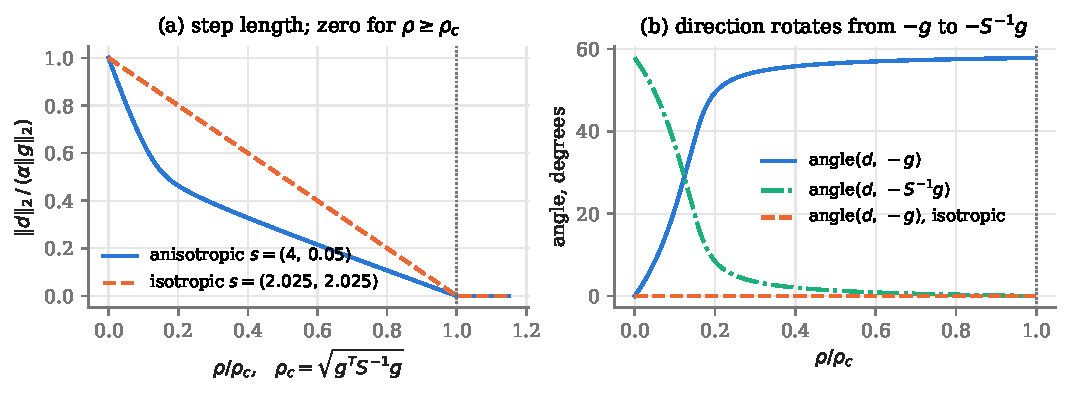
\includegraphics[width=\linewidth]{../fig/zero_step_sweep.pdf}
\caption{Robust step for $g=(1,\,0.6)$, $\alpha=0.5$ as a function of $\rho/\rho_c$.
Anisotropic $s=(4,\,0.05)$, $\rho_c=2.73$; isotropic $s$ with the same mean,
$\rho_c=0.82$. (a) Step length relative to SGD; it reaches zero exactly at
$\rho=\rho_c$. (b) Angle of $d$ to $-g$ and to $-S^{-1}g$; for isotropic $S$ the direction
never changes.}
\label{fig:sweep}
\end{figure}

\subsubsection*{Optimality condition of 1(d) and independent cross-checks}

\begin{center}
\begin{tabular}{@{}p{0.47\linewidth}p{0.45\linewidth}@{}}
\toprule
Check & Result \\
\midrule
Residual $r(d)$ of 1(d), 20\,000 random problems, $m\sim U(0.001,0.999)$ &
$\max r=1.0\cdot10^{-14}$ \\
Residual along all R-SGD trajectories of 4.5 & $\max r=9.9\cdot10^{-15}$ \\
Newton iterations, 20\,000 problems &
mean 4.4, median 4, 99\% quantile 7, max 9 \\
Safeguard bisections / non-monotone Newton iterates & $0$ / $0$ (5000 unsafeguarded runs) \\
Saddle point of (1): $d=-\alpha h^\star$,
$h^\star=g+\rho Sd/\sqrt{d^TSd}$ (part 1(a)) &
$\max\norm{d+\alpha h^\star}/\norm d=6.0\cdot10^{-12}$ \\
CVXPY (Clarabel), SOCP form, 300 problems ($s_j$ over four decades, $m\sim U(0.05,0.95)$) &
our objective never larger: $\max(\varphi_{\rm ours}-\varphi_{\rm cvx})/|\varphi|=1.8\cdot10^{-15}$ \\
& $\norm{d-d_{\rm cvx}}/\norm d$: median $4.0\cdot10^{-7}$, max $4.0\cdot10^{-4}$ \\
Strong-convexity certificate,
$\varphi(d+\delta)-\varphi(d)\ge\norm\delta^2/(2\alpha)$,
15\,000 random $\delta$ &
smallest relative slack $-1.6\cdot10^{-15}$ (rounding only) \\
\bottomrule
\end{tabular}
\end{center}

Remarks.
\begin{itemize}
\item The SOCP form used for CVXPY is
$\min_{d,t}\;g^Td+\rho t+\norm d^2/(2\alpha)$ s.t.\ $\norm{S^{1/2}d}\le t$. Its
solutions differ from ours by up to $4\cdot10^{-4}$ because an interior-point method
reaches only about $10^{-8}$ in the objective (Clarabel flagged 135 of 300 solves as
``optimal\_inaccurate'' at the requested tolerance $10^{-12}$). Since $\varphi$ is
$1/\alpha$-strongly convex, $\norm{d_{\rm cvx}-d^\star}^2\le2\alpha(\varphi(d_{\rm cvx})-\varphi(d^\star))$,
so an objective gap of $10^{-8}$ explains a distance of $10^{-4}$. Our objective was
never larger than CVXPY's.
\item The certificate test is a direct proof of optimality: for the exact minimiser of
a $1/\alpha$-strongly convex function the inequality holds for every $\delta$, and it
fails for small $\delta$ along a descent direction at any non-optimal point.
\item The saddle-point error is the residual measured differently:
$d+\alpha h^\star=\alpha\,(g+\rho Sd/\tau+d/\alpha)$, so it is amplified by
$\alpha\norm g/\norm d$, which is large just below the threshold.
\end{itemize}

\subsubsection*{Zero steps along trajectories of the noisy quadratic}

This is an illustration, not a tuned comparison: $b=8$, $\alpha_0=0.2$ (below
$2/L=0.5$), $\alpha_k=\alpha_0/\sqrt{1+k/50}$, $K=300$ updates, $\theta_0=(2,2)$, 20
seeds with common random numbers (both methods see the same $z_{k,i}$), and
$\rho\in\{1,\,2.45\}$. The value $2.45\approx\sqrt{\chi^2_{2,0.95}}$ is the radius at
which, for large $b$, 95\% of updates at the minimiser are zero steps (Section~\ref{sec:batch}).

\begin{center}
\begin{tabular}{@{}llcccc@{}}
\toprule
$\sigma$ & method & median final $f$ [IQR] & zero steps & max $f$ at a zero step & mean Newton it. \\
\midrule
0 & SGD & $6.3\cdot10^{-31}$ & -- & -- & -- \\
0 & R-SGD $\rho=1$ & $5.0\cdot10^{-12}$ & 0 & -- & 1.0 \\
0 & R-SGD $\rho=2.45$ & $3.0\cdot10^{-11}$ & 0 & -- & 1.0 \\
\midrule
1 & SGD & $0.0034$ [0.0020, 0.0067] & -- & -- & -- \\
1 & R-SGD $\rho=1$ & $0.0016$ [0.0005, 0.0073] & 33.0\% & 0.94 & 4.3 \\
1 & R-SGD $\rho=2.45$ & $0.0196$ [0.0085, 0.0386] & 80.8\% & 1.59 & 4.1 \\
\midrule
4 & SGD & $0.054$ [0.033, 0.107] & -- & -- & -- \\
4 & R-SGD $\rho=1$ & $0.026$ [0.008, 0.116] & 33.7\% & 2.50 & 4.3 \\
4 & R-SGD $\rho=2.45$ & $0.126$ [0.027, 0.269] & 85.0\% & 2.94 & 3.9 \\
\bottomrule
\end{tabular}
\end{center}

\begin{figure}[H]
\centering
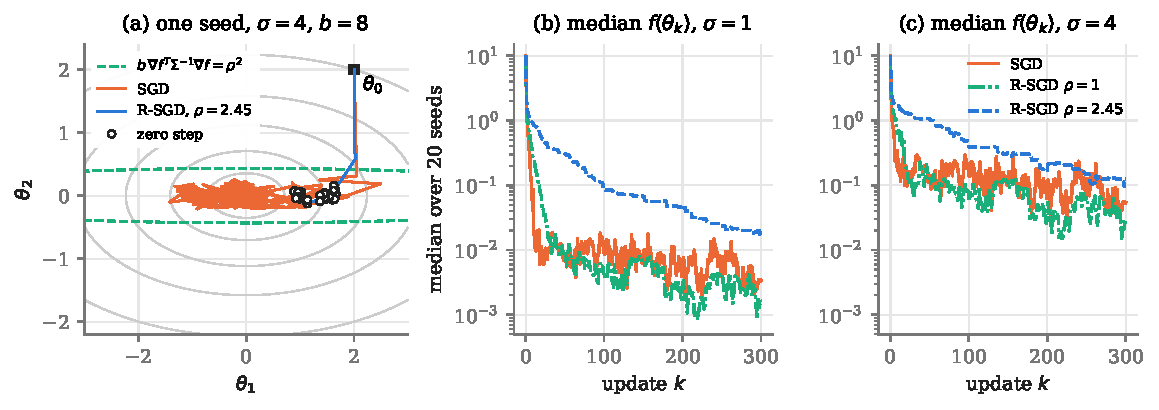
\includegraphics[width=\linewidth]{../fig/quadratic_trajectories.pdf}
\caption{Noisy quadratic, $b=8$, $\alpha_0=0.2$, 300 updates. (a) One seed at
$\sigma=4$: SGD and R-SGD ($\rho=2.45$) with identical noise draws; circles mark the
points where R-SGD took a zero step; the dashed ellipse is
$b\,\nabla f^T\Sigma^{-1}\nabla f=\rho^2$ (semi-axes $6.9$ and $0.43$, so in this window
it appears as a horizontal strip). (b), (c) Median of $f(\theta_k)$ over 20 seeds.}
\label{fig:traj}
\end{figure}

What these numbers show:
\begin{itemize}
\item \textbf{Zero steps happen far from the minimiser.} At $\sigma=4$, $\rho=2.45$,
zero steps occurred at points with $f$ up to $2.94$ (with $f(\theta_0)=10$ and
$f^\star=0$), where $\norm{\nabla f}$ is far from zero. Figure~\ref{fig:traj}(a) shows
why: along $\theta_1$ the gradient $\theta_1$ is weak and the noise (standard deviation
$2\sigma$ per observation) is strong, so the expected statistic
$b\,\nabla f^T\Sigma^{-1}\nabla f=b\big(\theta_1^2/(4\sigma^2)+64\theta_2^2/\sigma^2\big)$
stays below $\rho^2$ for $|\theta_1|$ up to $\rho\cdot2\sigma/\sqrt b=6.9$. R-SGD quickly
fixes $\theta_2$, whose signal-to-noise ratio is high, and then stalls in $\theta_1$.
This is the numerical counterpart of the answer to 1(c): (3) does not imply
$\nabla f(\theta_k)=0$.
\item \textbf{The $\varepsilon_k$ floor at $\sigma=0$.} All observations coincide,
$S_k=10^{-11}I$, and R-SGD converges to the boundary of its zero-step region,
$\norm{\nabla f}=\rho\sqrt{\varepsilon}$, where $f\approx\norm{\nabla f}^2/2=\rho^2\varepsilon/2$:
$5.0000\cdot10^{-12}$ for $\rho=1$ and $3.0013\cdot10^{-11}$ for $\rho=2.45$, matching
the measured medians to nine digits. The approach is continuous, which is why no exact
zero step was recorded. Since $S=\varepsilon I$ is isotropic, Newton took one iteration
at every update.
\item \textbf{A moderate radius can help; a large radius stalls.} $\rho=1$ lowered the
median final $f$ (0.0016 vs 0.0034 at $\sigma=1$; 0.026 vs 0.054 at $\sigma=4$), but the
interquartile ranges overlap, and $\rho=2.45$ was worse than SGD at both noise levels.
These are untuned illustration runs; whether the gain survives a fair tuning of
$\alpha_0$ for both methods, and whether it is more than a shorter step, is examined
in Sections~\ref{sec:protocol}--\ref{sec:critical}.
\item \textbf{Cost.} Both methods used $2400=bK$ gradient evaluations per run; the
wall-clock was about 4--7\,ms per run for SGD and 9--23\,ms for R-SGD (runs with many
zero steps are faster, since a zero step skips Newton).
\end{itemize}

\subsection{(c) Batch size and the uncertainty estimate}\label{sec:batch}

\subsubsection*{Theory}

Fix $\theta$ and let the observations be Gaussian, as in the quadratic:
$v_{i,j}\sim\mathcal N(\mu_j,\Sigma_{jj})$ i.i.d., with independent coordinates
($A$ diagonal). Standard facts about Gaussian samples give:
\begin{enumerate}
\item \textbf{Mean.} $\E\widehat s_j=\Sigma_{jj}/b$ (Section~\ref{sec:S}): the estimate itself
shrinks like $1/b$, because it estimates the variance of the mean.
\item \textbf{Spread.} $(b-1)\,b\,\widehat s_j/\Sigma_{jj}\sim\chi^2_{b-1}$, hence
$\operatorname{sd}(\widehat s_j)/\E\widehat s_j=\sqrt{2/(b-1)}$: 141\% at $b=2$, 53\% at
$b=8$, 9\% at $b=256$. With a small batch $S_k$ is itself very noisy.
\item \textbf{Zero-step statistic.} $g_j$ and $\widehat s_j$ are independent, and
$\E[1/\chi^2_\nu]=1/(\nu-2)$, so (neglecting $\varepsilon_k$)
\begin{align*}
\E\big[g^TS^{-1}g\big]&=\sum_j\E[g_j^2]\,\E[1/\widehat s_j]
=\sum_j\Big(\mu_j^2+\frac{\Sigma_{jj}}b\Big)\frac{b}{\Sigma_{jj}}\,\frac{b-1}{b-3}\\
&=\big(b\,\mu^T\Sigma^{-1}\mu+p\big)\frac{b-1}{b-3},\qquad b>3 .
\end{align*}
Away from a stationary point ($\mu\ne0$) the statistic grows \emph{linearly} in $b$, so
for fixed $\rho$ zero steps disappear as $b$ grows. At a stationary point ($\mu=0$)
each $g_j/\sqrt{\widehat s_j}$ is Student-$t$ with $b-1$ degrees of freedom, the mean is
$p(b-1)/(b-3)$, and for $b\le3$ it is infinite (heavy tails). For large $b$,
$g^TS^{-1}g\to\chi^2_p$ in distribution, which gives a natural scale for $\rho$:
$\rho=\sqrt{\chi^2_{p,0.95}}$ ($=2.45$ for $p=2$) means 95\% zero steps at the minimiser.
\item \textbf{Size of the robust correction.} The uncertainty radius in gradient
units is $\rho\sqrt{s_j}\propto\rho/\sqrt b$, so the shrinkage factors of 2.7 tend to 1
and R-SGD tends to SGD as $b\to\infty$ with $\rho$ fixed. In other words $\rho$ and $b$
are not independent knobs: the same $\rho$ means a different amount of robustness at
different batch sizes.
\end{enumerate}

\subsubsection*{Numerical check}

$\sigma=1$ (so $\Sigma=\diag(4,\tfrac14)$), $20\,000$ independent batches for each $b$,
at three fixed points: the minimiser $\theta^\star=(0,0)$, an intermediate point
$\theta_{\rm mid}=(1,\,0.1)$ with $\mu^T\Sigma^{-1}\mu=0.89$, and $\theta_0=(2,2)$ with
$\mu^T\Sigma^{-1}\mu=257$. Zero steps are counted for $\rho=2.45$; the last column is
the mean relative change of the step,
$\norm{d+\alpha g}/(\alpha\norm g)$, at $\theta_{\rm mid}$ for $\rho=1$, $\alpha=0.1$.

\begin{center}
\small
\setlength{\tabcolsep}{4.2pt}
\begin{tabular}{@{}rccccccccc@{}}
\toprule
& \multicolumn{2}{c}{$b\,\E\widehat s_j/\Sigma_{jj}$} & \multicolumn{2}{c}{rel.\ sd of $\widehat s_1$}
& \multicolumn{2}{c}{$\E\,g^TS^{-1}g$ at $\theta^\star$} & \multicolumn{2}{c}{zero-step freq.} & rel.\ change \\
\cmidrule(lr){2-3}\cmidrule(lr){4-5}\cmidrule(lr){6-7}\cmidrule(lr){8-9}
$b$ & $j=1$ & $j=2$ & emp. & $\sqrt{2/(b-1)}$ & emp. & theory & $\theta^\star$ & $\theta_{\rm mid}$ & at $\theta_{\rm mid}$ \\
\midrule
2 & 1.002 & 1.013 & 1.415 & 1.414 & 788.47 & $\infty$ & 0.558 & 0.410 & 0.579 \\
3 & 0.998 & 1.011 & 1.011 & 1.000 & 13.27 & $\infty$ & 0.719 & 0.484 & 0.606 \\
4 & 1.003 & 1.000 & 0.819 & 0.816 & 5.32 & 6.00 & 0.794 & 0.479 & 0.604 \\
8 & 0.994 & 0.999 & 0.534 & 0.535 & 2.78 & 2.80 & 0.885 & 0.297 & 0.536 \\
16 & 0.999 & 1.003 & 0.365 & 0.365 & 2.30 & 2.31 & 0.922 & 0.076 & 0.441 \\
32 & 0.998 & 1.003 & 0.251 & 0.254 & 2.14 & 2.14 & 0.938 & 0.001 & 0.338 \\
64 & 1.001 & 0.998 & 0.178 & 0.178 & 2.04 & 2.07 & 0.946 & 0.000 & 0.237 \\
128 & 0.999 & 1.000 & 0.126 & 0.125 & 2.02 & 2.03 & 0.946 & 0.000 & 0.167 \\
256 & 1.001 & 1.000 & 0.089 & 0.089 & 1.99 & 2.02 & 0.952 & 0.000 & 0.117 \\
\bottomrule
\end{tabular}
\end{center}
At $\theta_0$ the zero-step frequency was $0$ for every $b$.

\begin{figure}[H]
\centering
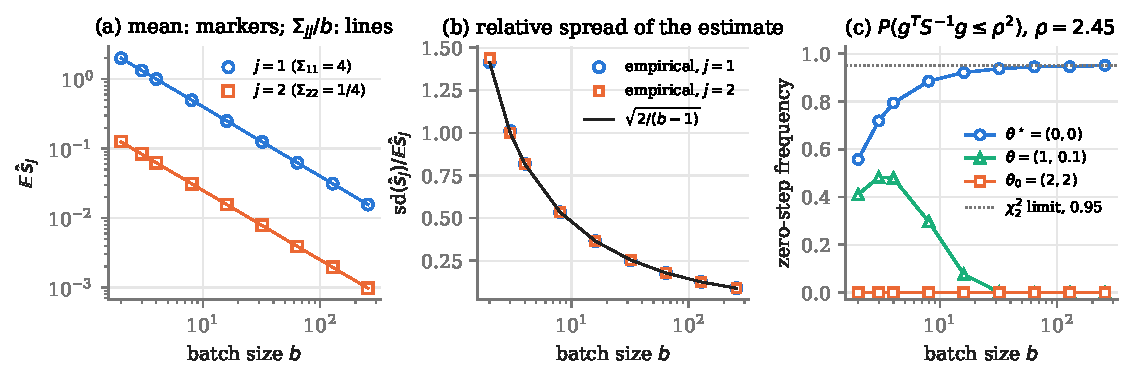
\includegraphics[width=\linewidth]{../fig/batch_size.pdf}
\caption{Batch size and the uncertainty estimate (noisy quadratic, $\sigma=1$,
$20\,000$ batches per $b$). (a) $\E\widehat s_j$ follows $\Sigma_{jj}/b$. (b) The
relative spread follows $\sqrt{2/(b-1)}$. (c) Zero-step frequency for $\rho=2.45$ at
three points; at $\theta^\star$ it tends to the $\chi^2_2$ value $0.95$.}
\label{fig:batch}
\end{figure}

Reading of the results:
\begin{itemize}
\item Points 1 and 2 of 5.1 are confirmed to within Monte Carlo error at every $b$
(ratios $1.00\pm0.013$; spreads within $0.025$ of $\sqrt{2/(b-1)}$).
\item The mean of $g^TS^{-1}g$ at $\theta^\star$ matches $p(b-1)/(b-3)$ for $b\ge8$. For
$b=2,3$ the theoretical mean is infinite and the sample means (788 and 13) are
meaningless; at $b=4$ the variance of the statistic is infinite, so the sample mean
converges slowly (5.3 vs 6.0). This is the heavy-tail effect of a two- or
three-point variance estimate.
\item At $\theta_{\rm mid}$ the zero-step frequency falls from about $0.4$--$0.5$ to
$0$ between $b=4$ and $b=32$: the transition happens where
$b\,\mu^T\Sigma^{-1}\mu\approx\rho^2$, i.e.\ $b\approx6/0.89\approx7$. The frequency is
\emph{not} monotone for $b\le4$: with very small batches $\widehat s_j$ is often tiny by
chance, $g^TS^{-1}g$ explodes and the zero step is avoided. Zero-step decisions at
$b\le4$ are therefore largely random.
\item The robust correction shrinks like $1/\sqrt b$: from $b=64$ to $b=256$ the
relative change halves ($0.237\to0.117$). With a fixed $\rho$, R-SGD at large $b$ is
nearly SGD.
\end{itemize}

\subsubsection*{Why sampling with replacement}

For the learning models the observations come from a finite training set of size $n$.
With replacement the $b$ draws are i.i.d.\ and $\E\widehat s_j=\Var(g_j)$ exactly.
Without replacement the variance of the batch mean has the finite-population factor
$(n-b)/(n-1)$, while the sample variance still estimates the population variance, so
$\widehat s_j$ overestimates $\Var(g_j)$ by the factor $n/(n-b)$. Check on a logistic
regression data set with $n=64$, $\sigma=0$, $20\,000$ batches:

\begin{center}
\begin{tabular}{@{}ccccc@{}}
\toprule
$n$ & $b$ & $\E\widehat s_j/\Var(g_j)$, with repl. & without repl. & predicted $n/(n-b)$ \\
\midrule
64 & 8 & 1.000--1.002 & 1.139--1.143 & 1.143 \\
64 & 32 & 0.999--1.003 & 2.000--2.004 & 2.000 \\
\bottomrule
\end{tabular}
\end{center}
(Ranges are over the three coordinates $w_1,w_2,c$.) Without replacement and with
$b=n/2$ the uncertainty would be overstated by a factor of 2, which would produce
spurious zero steps.

\subsection{(d) Implementation choices for reproduction}\label{sec:repro2}

\begin{itemize}
\item \textbf{Code.} \texttt{rsgd.py} (estimator (4), solver, SGD/R-SGD loop, oracles,
data generators, finite-difference check) and \texttt{checks\_section2.py} (every
number, table and figure of this section). Run: \texttt{python checks\_section2.py};
the full run takes about 20\,s.
\item \textbf{Random numbers.} One master seed $20261117$; the experiments use
independent child streams from \texttt{numpy.random.SeedSequence(20261117).spawn(8)}.
Inside an optimisation run there are two separate generators, one for batch indices
and one for gradient noise $z_{k,i}$ (in Section~\ref{sec:sims} also one for data and one for
initialisation).
\item \textbf{Common random numbers.} SGD and R-SGD are started from fresh generators
with the same seeds, so in a paired comparison they receive the same batch indices and
the same draws $z_{k,i}$ at every iteration (the observations still differ once the
iterates differ, since $u_i$ is evaluated at different $\theta_k$).
\item \textbf{Corruption model.} The noise is added only to the observations $V$.
The objective $f$, the training data, and all losses and accuracies are evaluated on
clean data.
\item \textbf{Settings.} float64 throughout; $b$, $\alpha_0$, schedule
$\alpha_0/\sqrt{1+k/50}$, number of updates $K$, $\rho$, $\sigma$, $\theta_0$ as stated in
each check; $\varepsilon_k$ exactly as in (4); solver tolerances
$|\psi|\le10^{-14}$, relative step $\le10^{-15}$, at most 100 iterations; a zero step is
recorded only when $g^TS^{-1}g\le\rho^2$.
\item \textbf{Reported per run.} Gradient evaluations ($bK$ for both methods),
wall-clock time, zero-step count, Newton iterations, maximum residual of 1(d).
\item \textbf{Software.} Python 3.13.18, NumPy 2.5.3, SciPy 1.18.1, Matplotlib 3.11.2,
CVXPY 1.9.3 (Clarabel) only for the cross-check.
\end{itemize}

\section{Required simulations}\label{sec:sims}

Both simulations compare SGD and R-SGD under the protocol of Section~\ref{sec:protocol}. The
settings selected there and then frozen for all noise levels are:
\begin{itemize}
\item logistic regression: SGD $\alpha_0=0.3$; R-SGD $\alpha_0=1$, $\rho=0.75\sqrt3=1.30$;
\item network: SGD $\alpha_0=1$; R-SGD $\alpha_0=10$, $\rho=0.25\sqrt{33}=1.44$.
\end{itemize}
All numbers come from \texttt{sim\_section3.py} (\texttt{results\_section3.json}) and all tables
from \texttt{make\_tables3.py}.

\subsection{Common setup}\label{sec:setup}


\begin{center}
\small
\begin{tabular}{@{}p{0.27\linewidth}p{0.68\linewidth}@{}}
\toprule
Item & Choice and reason \\
\midrule
Data & balanced classes; $n_{\rm train}=400$, $n_{\rm val}=400$, $n_{\rm test}=4000$ drawn
independently (large test set: the standard error of accuracy is $\le0.005$) \\
Preprocessing & standardisation $a\mapsto(a-\bar a_{\rm train})/s_{\rm train}$ with the
\emph{training} mean and standard deviation only, applied to all three sets \\
Loss & $\ell(t,y)=\log(1+e^t)-yt$, evaluated as \texttt{logaddexp(0,t)-y*t}; objective = mean
training loss, no regulariser; class $=\mathbf 1[t>0]$ \\
Batch and budget & $b=16$, sampling with replacement; $K=500$ updates (logistic), $K=3000$
(network); $bK$ gradient evaluations per run for both methods \\
Step sizes & $\alpha_k=\alpha_0/\sqrt{1+k/50}$ for both methods \\
Gradient noise & $v_{k,i}=u_i(\theta_k)+\sigma z_{k,i}$, $z_{k,i}\sim\mathcal N(0,I_p)$, i.i.d.\
across observations and iterations; $\sigma=c\,\gamma$, $c\in\{0,1,4,16\}$ \\
Noise unit $\gamma$ & RMS of the clean per-example gradients at the initial point, averaged
over the tuning seeds: $\gamma=0.500$ (logistic), $\gamma=0.215$ (network) \\
Uncertainty model & $g_k$, $S_k$ from formula (4) applied to the \emph{same} $b$ observations
used in the update \\
Evaluation & every loss and accuracy on clean data; 61 checkpoints per run for the curves \\
\bottomrule
\end{tabular}
\end{center}

\textbf{Noise levels.} $c=0$ is the case without artificial perturbation (mini-batch sampling
noise only). With $c=1$ the perturbation of one observation is as large as a typical
per-example gradient coordinate. With $c=4$ and $c=16$ it dominates. After averaging over
$b=16$ observations, the injected noise in $g_k$ has standard deviation $c\gamma/4$ per
coordinate.

\textbf{Radius scale.} The radius is parametrised as $\rho=r\sqrt p$. Near a stationary
point $g_k^TS_k^{-1}g_k$ is approximately $\chi^2_p$ with mean $p(b-1)/(b-3)$ (Section~\ref{sec:batch}), so the threshold of the zero-step rule scales with $\sqrt p$. A fixed $\rho$ would mean
very different things for $p=3$ and $p=33$; with $r$ the meaning is the same: $r\approx1$ is
the point where zero steps begin near a minimiser.

\subsection{Simulation 1: logistic regression}\label{sec:sim1}

\subsubsection*{Model, gradient and reference}

$a\mid y\sim\mathcal N\big((2y-1)(1,1)^T,I_2\big)$, $t_\theta(a)=w^Ta+c$, $\theta=(w_1,w_2,c)$,
$p=3$, $\theta_0=0$ (the problem is convex, so a fixed start is natural). The per-example
gradient is $u_i(\theta)=(\sigm(t_i)-y_i)\,(a_i^T,1)^T$ (Section~\ref{sec:oracles}). The
finite-difference check at the evaluation data gives relative errors $2.7\cdot10^{-10}$ (mean
gradient) and $1.9\cdot10^{-10}$ (per example).

\textbf{Reference.} The model is well specified: the log-likelihood ratio is
$\log\frac{p(a\mid1)}{p(a\mid0)}=2\,(1,1)a$, so the Bayes rule is $a_1+a_2>0$, with accuracy
$\Phi(\sqrt2)\approx0.921$. On the actual test sets of design A the Bayes rule has accuracy
$0.9228\pm0.0031$ and test loss $0.1905\pm0.0065$ (true logit $2(a_1+a_2)$). No method
can do better on average.

\subsubsection*{Results}

\begin{figure}[H]
\centering
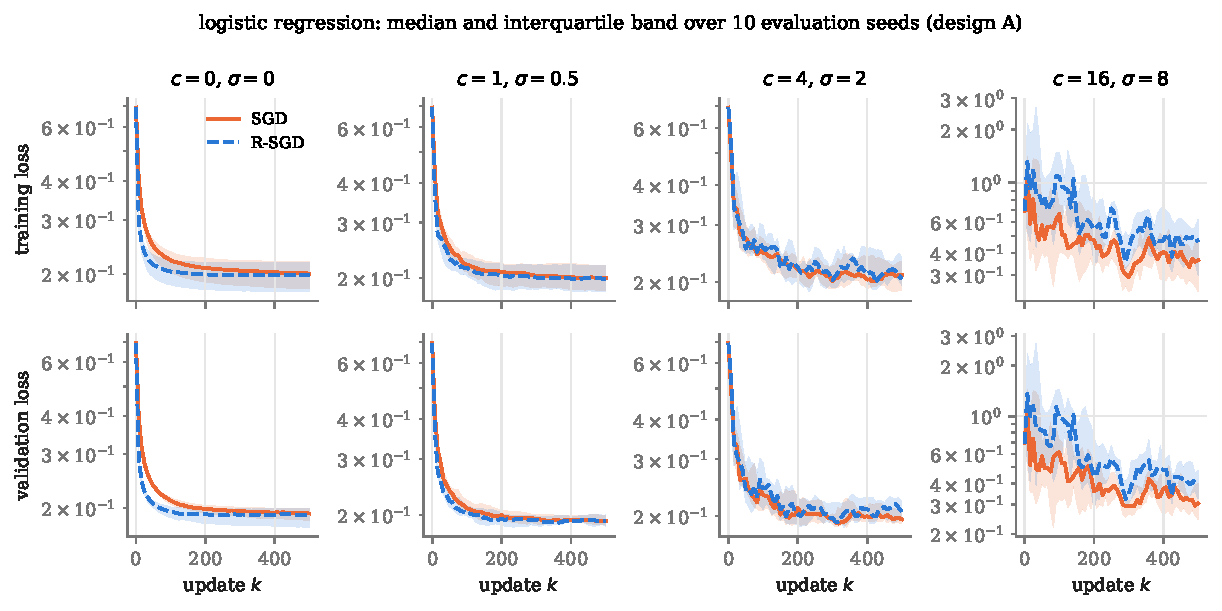
\includegraphics[width=\linewidth]{../fig3/logreg_curves.pdf}
\caption{Logistic regression: training (top) and validation (bottom) loss on clean data
against updates, median and interquartile band over 10 evaluation seeds (design A). Frozen
settings: SGD $\alpha_0=0.3$; R-SGD $\alpha_0=1$, $\rho=1.30$.}
\label{fig:lr_curves}
\end{figure}

\begin{center}
\small
\setlength{\tabcolsep}{4pt}
\begin{tabular}{@{}clccccc@{}}
\toprule
$c$ & method & final train loss & test loss & test accuracy & zero steps & time, ms (µs/update) \\
\midrule
\tabinput{../tabs3/tab_lr_main.tex}
\bottomrule
\end{tabular}

\smallskip
Logistic regression, design A, mean $\pm$ sd over 10 seeds; $bK=8000$ gradient evaluations per
run for both methods; Bayes rule: accuracy $0.9228$, test loss $0.1905$.
\end{center}

\begin{center}
\small
\setlength{\tabcolsep}{2.6pt}
\begin{tabular}{@{}cccccccccc@{}}
\toprule
& & \multicolumn{2}{c}{$\Delta$ train loss} & \multicolumn{2}{c}{$\Delta$ test loss}
& \multicolumn{2}{c}{$\Delta$ accuracy} & \multicolumn{2}{c}{ranking agreement} \\
\cmidrule(lr){3-4}\cmidrule(lr){5-6}\cmidrule(lr){7-8}\cmidrule(lr){9-10}
$c$ & design & mean $\pm$ h & wins & mean $\pm$ h & wins & mean $\pm$ h & wins (ties) & tr$\to$te & tr$\to$acc \\
\midrule
\tabinput{../tabs3/tab_lr_paired.tex}
\bottomrule
\end{tabular}

\smallskip
Paired differences R-SGD $-$ SGD (negative loss and positive accuracy differences favour
R-SGD); ``ranking agreement'': number of seeds in which the sign of $\Delta$ train loss
predicts the sign of $\Delta$ test loss (tr$\to$te) or of $-\Delta$ accuracy (tr$\to$acc).
\end{center}

Reading.
\begin{itemize}
\item \textbf{Accuracy is saturated.} At $c\le4$ both methods are within $0.005$ of the Bayes
accuracy, and the mean accuracy difference is below $0.001$ in absolute value. Loss differences
of a few thousandths move the linear boundary by a negligible amount
(Figure~\ref{fig:lr_bound}).
\item \textbf{Small, consistent loss gain at $c\le1$.} Within a fixed data set (design B) R-SGD
has a lower training loss in 10/10 ($c=0$) and 9/10 ($c=1$) seeds and lower test loss in 10/10
and 8/10. Across data sets (design A) the same differences are hidden by the much larger
data-set spread (sd of test loss $0.007$ in A vs.\ $0.001$ in B at $c=0$).
\item \textbf{Worse at $c\ge4$ with frozen settings.} R-SGD runs with $\alpha_0=1$, three times
SGD's step size, and relies on shrinkage to compensate. When noise dominates, the shrinkage is
nearly a constant factor (Section~\ref{sec:critical}(a)), large noisy gradients pass through, and the loss is higher:
$+0.005$ at $c=4$ and $+0.095$ at $c=16$, SGD better in 7--8 of 10 seeds.
\item \textbf{Zero steps:} 18\% of updates at $c=0$ and 32--33\% at $c\ge1$, including
updates early in training. They did not prevent convergence because $p=3$ and the remaining steps
are large.
\item \textbf{Runtime:} SGD 16--21\,µs per update, R-SGD 58--88\,µs (2.8--4.4 times more),
with identical gradient-evaluation counts.
\end{itemize}

\begin{figure}[H]
\centering
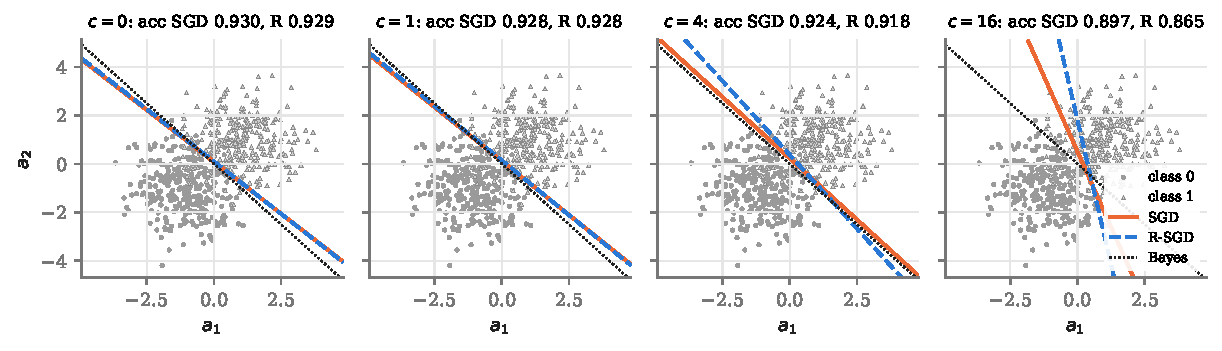
\includegraphics[width=\linewidth]{../fig3/logreg_boundaries.pdf}
\caption{Logistic regression, evaluation seed A-0 (seeds in Section~\ref{sec:repro}): decision
boundaries $t_\theta(a)=0$ of the final SGD and R-SGD iterates in original coordinates, the
Bayes boundary $a_1+a_2=0$, and 600 test points.}
\label{fig:lr_bound}
\end{figure}

\subsection{Simulation 2: two-layer network}\label{sec:sim2}

\subsubsection*{Model, initialisation, gradient}

Semicircles: $t\sim U[0,\pi]$, class 0 at $(\cos t,\sin t)+e$, class 1 at
$(1-\cos t,\tfrac12-\sin t)+e$, $e\sim\mathcal N(0,0.1^2I_2)$. Model
$t_\theta(a)=w_2^T\tanh(W_1a+b_1)+b_2$ with 8 hidden units, $p=33$. Initialisation:
$W_1\sim\mathcal N(0,\tfrac12)$, $b_1=0$, $w_2\sim\mathcal N(0,\tfrac18)$, $b_2=0$ (variance
$1/\text{fan-in}$), drawn from the seed's initialisation stream; SGD and R-SGD start from the
same $\theta_0$. The initial loss is close to $\log2=0.693$. The gradient is computed by
per-example back-propagation (Section~\ref{sec:oracles}); the finite-difference check at the actual
initial point gives relative errors $4.9\cdot10^{-10}$ (mean) and $8.9\cdot10^{-10}$ (per
example).

\subsubsection*{Results}

\begin{figure}[H]
\centering
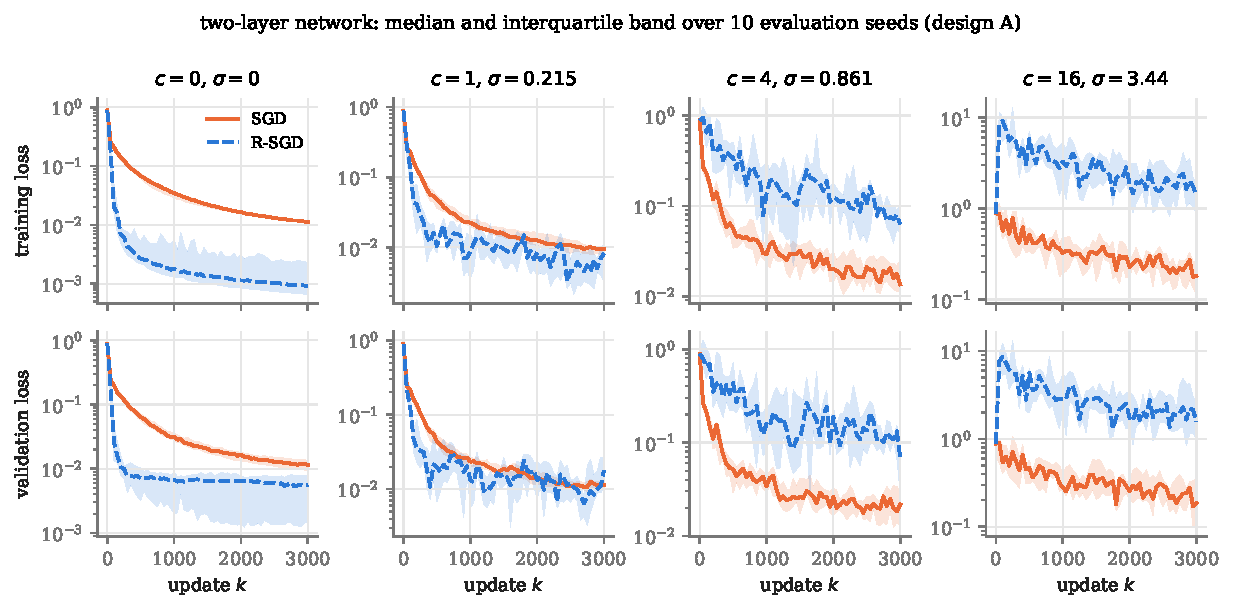
\includegraphics[width=\linewidth]{../fig3/mlp_curves.pdf}
\caption{Two-layer network: training (top) and validation (bottom) loss on clean data, median
and interquartile band over 10 evaluation seeds (design A). Frozen settings: SGD $\alpha_0=1$;
R-SGD $\alpha_0=10$, $\rho=1.44$.}
\label{fig:mlp_curves}
\end{figure}

\begin{center}
\small
\setlength{\tabcolsep}{4pt}
\begin{tabular}{@{}clccccc@{}}
\toprule
$c$ & method & final train loss & test loss & test accuracy & zero steps & time, ms (µs/update) \\
\midrule
\tabinput{../tabs3/tab_mlp_main.tex}
\bottomrule
\end{tabular}

\smallskip
Two-layer network, design A, mean $\pm$ sd over 10 seeds; $bK=48\,000$ gradient evaluations per
run for both methods.
\end{center}

\begin{center}
\small
\setlength{\tabcolsep}{2.6pt}
\begin{tabular}{@{}cccccccccc@{}}
\toprule
& & \multicolumn{2}{c}{$\Delta$ train loss} & \multicolumn{2}{c}{$\Delta$ test loss}
& \multicolumn{2}{c}{$\Delta$ accuracy} & \multicolumn{2}{c}{ranking agreement} \\
\cmidrule(lr){3-4}\cmidrule(lr){5-6}\cmidrule(lr){7-8}\cmidrule(lr){9-10}
$c$ & design & mean $\pm$ h & wins & mean $\pm$ h & wins & mean $\pm$ h & wins (ties) & tr$\to$te & tr$\to$acc \\
\midrule
\tabinput{../tabs3/tab_mlp_paired.tex}
\bottomrule
\end{tabular}

\smallskip
Two-layer network: paired differences R-SGD $-$ SGD, as in the logistic-regression table.
\end{center}

Reading.
\begin{itemize}
\item \textbf{$c=0$: R-SGD optimises faster.} Its training loss is $0.0019$ vs.\ $0.0110$
(10/10 seeds in both designs); test loss is lower in 9/10 (A) and 10/10 (B). The curves in
Figure~\ref{fig:mlp_curves} separate after a few hundred updates. Accuracy is not better (3 wins,
2 ties), because both methods already classify $99.8\%$ of the test points correctly.
\item \textbf{The $c=0$ gain is a step-length gain.} R-SGD's mean step ratio is $0.59$, so it
moves like SGD with $\alpha_0'=5.9$, six times SGD's tuned $1$. That SGD run reaches test loss
$0.0065$ vs.\ R-SGD's $0.0082$ (R-SGD better in 4/10). SGD's $\alpha_0=1$ was chosen at $c=1$
from a noisy criterion, not at $c=0$.
\item \textbf{$c=1$, the tuning level itself: R-SGD is worse.} Its evaluation validation loss is
$0.0230\pm0.0207$ against SGD's $0.0114\pm0.0028$, although tuning had predicted the opposite
($0.0104$ vs.\ $0.0138$). The R-SGD selection was the minimum of 36 noisy estimates against 6 for
SGD, which makes it optimistically biased (the ``winner's curse''), and the chosen large
$\alpha_0=10$ is a high-variance setting. Test accuracy: $0.9946$ vs.\ $0.9980$, SGD better in
8 of 10 seeds (one tie).
\item \textbf{$c\ge4$: the frozen R-SGD setting breaks down.} Test loss $0.115$ vs.\ $0.025$
($c=4$) and $1.96$ vs.\ $0.22$ ($c=16$); at $c=16$, 8 of 10 R-SGD runs end with a training loss
above the initial $\log2$. An effective step size of about $7.4/\sqrt{1+k/50}$, i.e.\ 7.4 times
SGD's, with noise-dominated gradients throws the network into saturated regions. No run met the formal failure criterion (loss $>50$
times the initial loss).
\item \textbf{Zero steps:} none at the selected $\rho=1.44$, which is far below the
noise-dominated threshold $\approx\sqrt{p(b-1)/(b-3)}=6.2$.
\item \textbf{Runtime:} SGD 32--49\,µs per update, R-SGD 109--128\,µs (2.6--3.6 times more).
\end{itemize}

\begin{figure}[H]
\centering
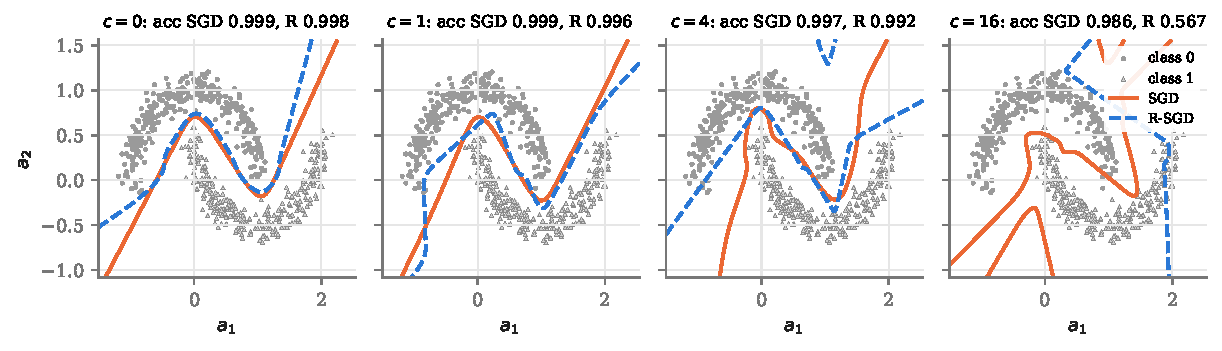
\includegraphics[width=\linewidth]{../fig3/mlp_boundaries.pdf}
\caption{Two-layer network, evaluation seed A-0: decision boundaries of the final SGD and R-SGD
iterates in original coordinates with 600 test points. Away from the data the two boundaries
extrapolate differently even when both separate the semicircles (left two panels).}
\label{fig:mlp_bound}
\end{figure}

\subsection{Do optimisation and prediction give the same ranking?}\label{sec:ranking}

\begin{itemize}
\item \textbf{Training loss vs.\ test loss: mostly yes.} Within a fixed data set (design B) the
sign of $\Delta$ train loss predicted the sign of $\Delta$ test loss in 7--10 of 10 seeds in all
cases except the network at $c=1$ (3/10). In design A the exceptions are the network at $c=1$
(5/10) and logistic regression at $c=0$ (2/10), where differences of $0.002$ are swamped by the
variation between data sets. Both data sets are simple, and with 400 training points the models
are far from overfitting.
\item \textbf{Training loss vs.\ accuracy: no at low noise.} Logistic regression at $c\le1$:
agreement 3--5/10; the network at $c=0$: 3/10, although R-SGD's training loss is 5.8 times
smaller. Lower cross-entropy here mostly means more confident logits on points that are already
correctly classified. Logistic regression is at the Bayes accuracy, so no optimiser can improve
accuracy; for the network both methods are at $99.8\%$.
\item \textbf{At high noise all rankings agree} (7--10/10): the noise damages the boundary
itself, and the method with the smaller loss also classifies better.
\item For the two simulations together: lower training loss, lower test loss and higher
accuracy are different outcomes, as the assignment's success criterion states. In these
experiments R-SGD sometimes achieved the first two; it never achieved a higher accuracy than an
SGD run with the same mean step length.
\end{itemize}

\section{Fair tuning and evaluation}\label{sec:protocol}

\subsection{Comparable budgets}
Both methods use the same batch size $b=16$ (sampling with replacement), the same number of updates
($K=500$ for logistic regression, $K=3000$ for the network) and the same schedule
$\alpha_k=\alpha_0/\sqrt{1+k/50}$. Every run therefore uses exactly $bK$ per-example gradient
evaluations: $8000$ and $48\,000$ respectively, identical for SGD and R-SGD. Runtime is measured
over the $K$ updates only, excluding the evaluation checkpoints, and reported in the result tables
of Section~\ref{sec:sims}. In Python R-SGD costs 2.6--4.4 times more per update, because of the
solver's fixed overhead. The comparison is between plain SGD and R-SGD only.

\subsection{Hyperparameter selection}\label{sec:tuning}
\textbf{Tuning protocol.}
\begin{itemize}
\item Grids: $\alpha_0\in\{0.1,0.3,1,3,10,30\}$ for both methods; $r\in\{0,0.25,0.5,0.75,1,1.25\}$
for R-SGD. $r=0$ is included, and R-SGD with $r=0$ is SGD.
\item Tuning data: 3 tuning seeds with their own data sets, initialisations, batches and noise,
disjoint from all evaluation seeds; tuning noise level $c=1$. Test data are never used.
\item Criterion: mean over tuning seeds of the validation loss averaged over the last 5 of 61
checkpoints. A run is marked failed if its training loss becomes non-finite or exceeds 50 times
its initial value.
\item Search budgets: SGD $6\times3=18$ runs, R-SGD $36\times3=108$ runs. The larger R-SGD
budget favours R-SGD (it is the minimum over more noisy estimates); this is discussed below.
\item Settings are frozen after tuning and then used unchanged at every noise level.
\end{itemize}

\paragraph{Logistic regression.}
\begin{figure}[H]
\centering
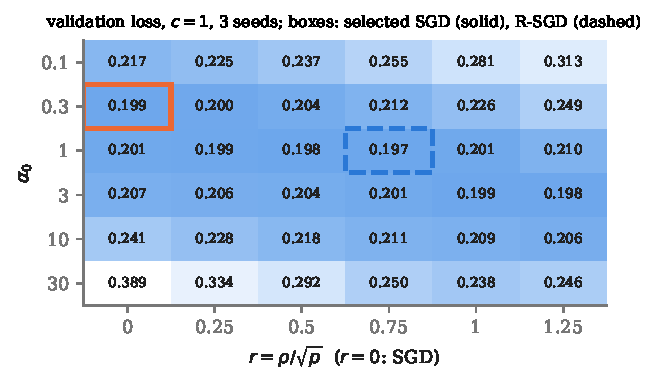
\includegraphics[width=0.49\linewidth]{../fig3/logreg_tuning.pdf}\hfill
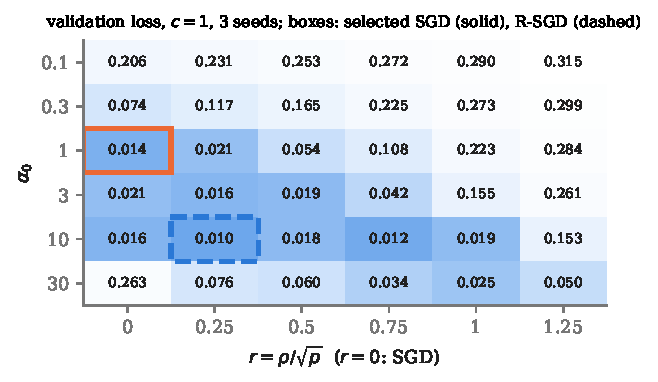
\includegraphics[width=0.49\linewidth]{../fig3/mlp_tuning.pdf}
\caption{Tuning criterion (mean validation loss, $c=1$, 3 tuning seeds) for logistic regression
(left) and the network (right). Column $r=0$ is SGD. Boxes mark the selected settings.}
\label{fig:tuning}
\end{figure}

Selected: SGD $\alpha_0=0.3$; R-SGD $\alpha_0=1$, $r=0.75$ ($\rho=1.30$). Neither lies on the
edge of the grid. The criterion is very flat: 10 of 36 cells are within $0.005$ of the best
($0.197$). The low region runs along a diagonal: a larger $\alpha_0$ is compensated by a larger
$r$, e.g.\ $(1,0.75)$, $(3,1)$, $(3,1.25)$ are almost equal. This is the trade-off between
learning rate and radius asked about in Section 5(b): both control the effective step length.

\paragraph{Network.}
Selected (Figure~\ref{fig:tuning}, right): SGD $\alpha_0=1$; R-SGD $\alpha_0=10$, $r=0.25$
($\rho=1.44$). Neither is on the edge. The R-SGD criterion ($0.0104$) is below SGD's
($0.0138$), but the surface is irregular: $(10,0)$, i.e.\ SGD with $\alpha_0=10$, has $0.0156$,
$(10,0.5)$ has $0.0184$, $(10,0.75)$ has $0.0117$. Such non-monotone neighbours indicate that
differences of this size are within the noise of a 3-seed estimate. Section~\ref{sec:sim2} shows the
consequence.

\subsection{Reproducibility and variability}\label{sec:variability}
\textbf{Evaluation designs.} Two designs, each with 10 seeds, paired across methods
(same data, initialisation, batch indices and noise draws $z_{k,i}$):
\begin{itemize}
\item \textbf{A} (data set varies): every seed draws a new training, validation and test set,
a new initialisation, new batches and new noise. Spread in A combines uncertainty across data
sets and training randomness.
\item \textbf{B} (training randomness only): the data set of A-seed 0 is fixed; initialisation,
batches and noise vary.
\end{itemize}
Error bars: ``mean $\pm$ sd'' is the mean and the sample standard deviation over the 10 seeds
(the spread of outcomes). For paired differences ``mean $\pm$ h'' gives the half-width $h$ of
the 95\% $t$-interval for the mean difference, and ``wins'' counts seeds where R-SGD is better
(ties in parentheses).

\paragraph{Logistic regression.}
\begin{center}
\small
\begin{tabular}{@{}ccccccccc@{}}
\toprule
& \multicolumn{4}{c}{sd of test loss} & \multicolumn{4}{c}{sd of test accuracy} \\
\cmidrule(lr){2-5}\cmidrule(lr){6-9}
$c$ & SGD A & SGD B & R-SGD A & R-SGD B & SGD A & SGD B & R-SGD A & R-SGD B \\
\midrule
\tabinput{../tabs3/tab_lr_var.tex}
\bottomrule
\end{tabular}

\smallskip
Logistic regression: spread across data sets and training randomness (A) versus training
randomness only (B).
\end{center}
At $c\le1$ the spread across data sets dominates (the sd in A is 2--7 times that in B); at
$c\ge4$ the injected noise makes training randomness the main source.

\paragraph{Network.}
\begin{center}
\small
\begin{tabular}{@{}ccccccccc@{}}
\toprule
& \multicolumn{4}{c}{sd of test loss} & \multicolumn{4}{c}{sd of test accuracy} \\
\cmidrule(lr){2-5}\cmidrule(lr){6-9}
$c$ & SGD A & SGD B & R-SGD A & R-SGD B & SGD A & SGD B & R-SGD A & R-SGD B \\
\midrule
\tabinput{../tabs3/tab_mlp_var.tex}
\bottomrule
\end{tabular}

\smallskip
Two-layer network: spread across data sets and training randomness (A) versus training
randomness only (B).
\end{center}
For the network the spread in B (training randomness including the initialisation) is
comparable to the spread in A, unlike logistic regression: the non-convex model is sensitive to
its initialisation and to the trajectory. With 10 seeds an sd is itself uncertain by about
$\pm25\%$, so only large ratios are meaningful.

No run met the failure criterion (training loss non-finite or above 50 times its initial value) in
tuning, evaluation or the sweep. The 8 network runs at $c=16$ whose final loss exceeded the initial
$\log2$ are reported in Section~\ref{sec:sim2}.

\subsection{Sensitivity and step length}\label{sec:sens}
\textbf{Sensitivity study and control.} (i) A radius sweep $r\in\{0,\dots,2\}$ at SGD's tuned $\alpha_0$,
5 seeds. (ii) A step-length-matched SGD control: SGD with
$\alpha_0'=\alpha_0\cdot\overline{\|d_k\|/(\alpha_k\|g_k\|)}$, the mean step ratio of the
corresponding R-SGD runs (zero steps count as 0). It is run for the frozen setting and for every
point of the sweep, on the same seeds.

\paragraph{Logistic regression.}
\begin{center}
\small
\setlength{\tabcolsep}{4pt}
\begin{tabular}{@{}cccccccc@{}}
\toprule
$c$ & step ratio & $\alpha_0'$ & R-SGD test loss & matched SGD test loss & $\Delta$ (R $-$ matched) & wins & acc R / matched \\
\midrule
\tabinput{../tabs3/tab_lr_matched.tex}
\bottomrule
\end{tabular}

\smallskip
Frozen R-SGD versus SGD with the same mean step length, design A, 10 seeds.
\end{center}

At $c=0$ the matched step size is exactly SGD's tuned $0.3$, and the two methods tie (5/10).
At $c=1$, R-SGD beats the matched SGD in 9/10 seeds by $0.003$ in test loss. At $c\ge4$ the
matched SGD is better, at $c=16$ by $0.14$.

\begin{figure}[H]
\centering
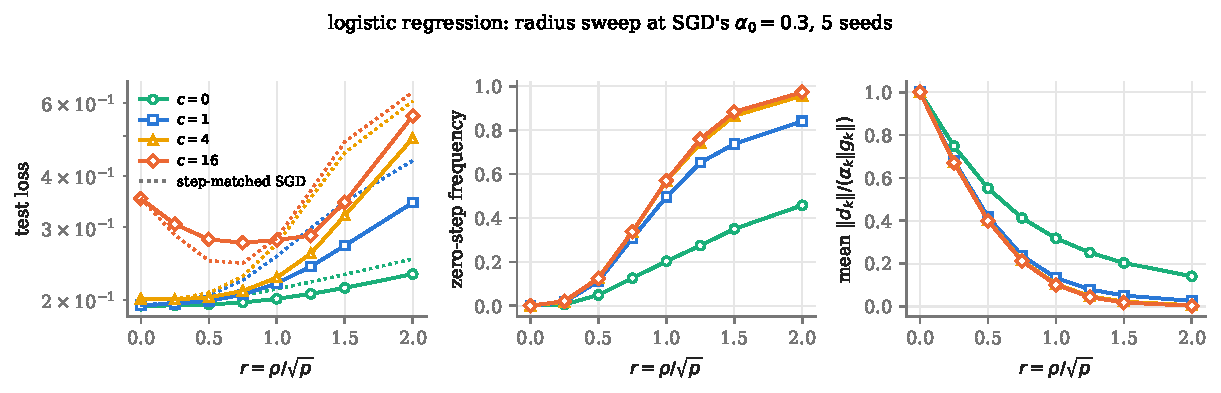
\includegraphics[width=\linewidth]{../fig3/logreg_sensitivity.pdf}
\caption{Logistic regression, radius sweep at SGD's $\alpha_0=0.3$, 5 seeds. Left: test loss of
R-SGD (solid) and of step-length-matched SGD (dotted). Middle: zero-step frequency. Right: mean
step ratio $\|d_k\|/(\alpha_k\|g_k\|)$.}
\label{fig:lr_sens}
\end{figure}

\begin{center}
\small
\setlength{\tabcolsep}{4pt}
\begin{tabular}{@{}ccccccccc@{}}
\toprule
$c$ & $r$ & zero steps & step ratio & train loss & test loss & matched SGD test & R wins & test acc \\
\midrule
\tabinput{../tabs3/tab_lr_sens.tex}
\bottomrule
\end{tabular}

\smallskip
Logistic regression, radius sweep at $\alpha_0=0.3$ (means over 5 seeds); $r=0$ is SGD.
\end{center}

\begin{itemize}
\item At $c\le4$, increasing $r$ does not lower the loss (at most by $0.0007$ for $r=0.25$,
then it rises): with a tuned SGD step there is nothing to gain. But R-SGD is better than SGD
with the same mean step at every $r$, in 5/5 seeds (4/5 once). Its shrinkage is small early (large gradients, high signal-to-noise ratio) and
large late, i.e.\ it acts as an adaptive decay of the step size; a constant reduction loses
speed early.
\item At $c=16$, $r=0.5$--$0.75$ lowers the test loss from $0.352$ to $0.275$, but the matched SGD
does better ($0.246$, R-SGD wins 1/5): the gain is a step-length effect.
\item Accuracy hardly changes with $r$ (within $0.002$ at $c\le4$) until zero steps dominate.
\end{itemize}

\paragraph{Network.}
\begin{center}
\small
\setlength{\tabcolsep}{4pt}
\begin{tabular}{@{}cccccccc@{}}
\toprule
$c$ & step ratio & $\alpha_0'$ & R-SGD test loss & matched SGD test loss & $\Delta$ (R $-$ matched) & wins & acc R / matched \\
\midrule
\tabinput{../tabs3/tab_mlp_matched.tex}
\bottomrule
\end{tabular}

\smallskip
Two-layer network: frozen R-SGD versus SGD with the same mean step length, design A, 10 seeds.
\end{center}

\begin{figure}[H]
\centering
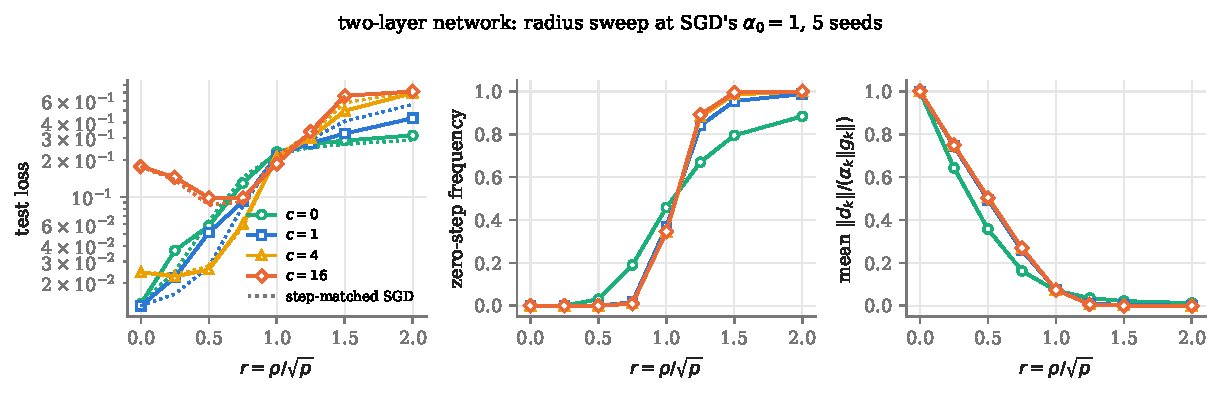
\includegraphics[width=\linewidth]{../fig3/mlp_sensitivity.pdf}
\caption{Two-layer network, radius sweep at SGD's $\alpha_0=1$, 5 seeds. Left: test loss of
R-SGD (solid) and of step-length-matched SGD (dotted). Middle: zero-step frequency. Right: mean
step ratio.}
\label{fig:mlp_sens}
\end{figure}

\begin{center}
\small
\setlength{\tabcolsep}{4pt}
\begin{tabular}{@{}ccccccccc@{}}
\toprule
$c$ & $r$ & zero steps & step ratio & train loss & test loss & matched SGD test & R wins & test acc \\
\midrule
\tabinput{../tabs3/tab_mlp_sens.tex}
\bottomrule
\end{tabular}

\smallskip
Two-layer network, radius sweep at $\alpha_0=1$ (means over 5 seeds); $r=0$ is SGD.
\end{center}

\begin{itemize}
\item At $c\le1$ every $r>0$ worsens the result; at $c=4$ the effect of $r\le0.5$ is within
noise.
\item At $c=16$, $r=0.5$--$0.75$ improves the test loss from $0.176$ to $0.098$ and the
accuracy from $0.953$ to $0.968$, but the matched SGD is better still ($0.086$; R-SGD wins
2/5 and 1/5). In the noise-dominated regime the robust step behaves as a shorter SGD step.
\item \textbf{Zero steps before a minimiser.} For $r\ge1$ the zero-step frequency jumps to
35--100\%, and training stops at test accuracy $0.91$--$0.50$. At $c=4,16$ with $r=2$ the
network practically never moves (99.9--100\% zero steps, accuracy $0.50$). The
explanation (Section~\ref{sec:critical}(b)): when noise dominates, $g_k^TS_k^{-1}g_k$ is close to its value at a
stationary point regardless of $\theta_k$, so the zero-step test cannot tell whether the iterate
is near a minimiser.
\end{itemize}

\paragraph{Conclusion of the sensitivity study.} Increasing the radius mostly shortens the step.
Wherever R-SGD improved on SGD in the sweep, an SGD run with the same mean step length did as well
or better, except in logistic regression at $c\le4$. There R-SGD's signal-to-noise-dependent
shrinkage beat a constant step reduction, on loss only. Radii $\rho\gtrsim\sqrt p$ produce zero
steps far from any minimiser (Section~\ref{sec:critical}).


\section{Critical analysis}\label{sec:critical}

The answers below separate three kinds of statement: mathematical results (Section~1),
mechanisms derived under stated assumptions, and empirical findings for our two problems and
settings.

\subsection{(a) When does R-SGD help?}

\textbf{Evidence for a benefit.}
\begin{itemize}
\item \emph{Low noise, logistic regression.} R-SGD lowered the loss slightly but consistently. At
$c=1$ its test loss was $0.0027$ below that of SGD run with the same mean step length in 9/10
seeds. In the radius sweep at $c\le4$ it beat the step-matched SGD at every radius, in 5/5 seeds (4/5 once).
Here the per-coordinate variances differ and change over time, so the shrinkage acts as an
adaptive, signal-to-noise-driven step decay. It is weak early, when gradients are large and
reliable, and strong near the minimiser. A constant step reduction of the same mean cannot
reproduce this.
\item \emph{A safeguard for large step sizes at low noise.} Tuning chose larger step sizes for
R-SGD ($3\times$ and $10\times$ SGD's), which its shrinkage made usable at $c\le1$. On the network
at $c=0$ this gave $5.8\times$ lower training loss than the tuned SGD.
\end{itemize}

\textbf{Evidence against.}
\begin{itemize}
\item That network gain is a step-length gain. SGD with R-SGD's mean step length reached the same
training loss ($0.0018$ vs.\ $0.0019$) and a lower test loss ($0.0065$ vs.\ $0.0082$).
\item No accuracy gain anywhere: logistic regression is at the Bayes accuracy, and the network at
$99.8\%$.
\item With noise, the frozen R-SGD settings were worse than SGD in both simulations, and in the
sweep every R-SGD improvement at $c=16$ was matched or beaten by step-matched SGD.
\end{itemize}

\textbf{Mechanism (derived, then confirmed).} When the injected noise dominates, all
$\widehat s_{k,j}\approx\sigma^2/b$, so $S_k\approx sI$ and part 1(d) applies. Since $g_k$ is
mostly noise, $\norm{g_k}^2\approx ps$, and with $\rho=r\sqrt p$
\begin{equation*}
\frac{\norm{d_k}}{\alpha_k\norm{g_k}}\approx1-\frac{\rho\sqrt s}{\sqrt{ps}}=1-r .
\end{equation*}
Measured on the network at $c\ge4$: $0.748,\ 0.505,\ 0.269$ for $r=0.25,0.5,0.75$. For $p=3$ the
values are rougher ($0.67, 0.40, 0.21$), because $\norm{g_k}$ fluctuates more in three dimensions.
In this regime R-SGD is, to first order, SGD with a shorter step and the same direction, so it
should not beat an SGD whose step size is tuned at that noise level. To second order it is worse
than a constant reduction: $1-\rho\sqrt s/\norm{g_k}$ grows with $\norm{g_k}$, so the largest,
noisiest gradients are shrunk least. The robust step soft-thresholds the gradient norm; it does not
reduce variance.

\textbf{Answer.} In these experiments R-SGD helped only when (i) the uncertainty was anisotropic
and varied over time, so its shrinkage differed from a constant step reduction; (ii) the estimate
$S_k$ was reliable ($b\ge8$); and (iii) the measure was loss, not accuracy. Under dominant
isotropic noise it reduces to a shorter SGD step and cannot beat a tuned SGD.

\subsection{(b) Interactions among radius, covariance and learning rate}

\begin{itemize}
\item \textbf{Radius and learning rate both set the step length.} For a nonzero step,
$d_{k,j}=-\alpha_k\,\tau g_{k,j}/(\tau+\alpha_k\rho s_{k,j})$ depends on the product
$\alpha_k\rho s_{k,j}$. The tuning surfaces show the trade-off: in logistic regression the
near-optimal cells lie on a diagonal, with $(\alpha_0,r)=(1,0.75)$, $(3,1)$ and $(3,1.25)$ almost
equal (Figure~\ref{fig:tuning}). A larger step size is compensated by a larger radius.
\item \textbf{The zero-step decision does not depend on $\alpha_k$} (Section~1(c)). It depends
only on $\rho$ and $S_k$. So $\alpha$ scales the nonzero steps, while $\rho$ alone decides where
the method stops moving.
\item \textbf{Covariance scales with the batch and the noise.} $S_k\approx\Sigma/b$, where $\Sigma$
includes the sampling variance and $\sigma^2I$. The uncertainty radius in gradient units,
$\rho\sqrt{s_{k,j}}$, therefore scales like $\rho\sigma/\sqrt b$ under noise. The robust correction
fades as $1/\sqrt b$: it fell from $0.237$ to $0.117$ between $b=64$ and $b=256$ (Section~2). The
same $\rho$ means different robustness at different batch sizes and noise levels, which is why
$\rho$ must be tuned at the batch size used. The scale $\rho=r\sqrt p$ makes it comparable across
models.
\item \textbf{Zero steps before reaching a minimiser.} With exact $S=\Sigma/b$, zero steps occur
roughly where $b\,\nabla f^T\Sigma^{-1}\nabla f\le\rho^2$. This region surrounds the minimiser
but extends far along low-curvature, high-noise directions. On the noisy quadratic
($\sigma=4$, $b=8$, $\rho=2.45$) its semi-axes are $6.9$ and $0.43$, and zero steps occurred at
$f$ up to $2.94$ ($f(\theta_0)=10$). Under heavy injected noise,
$g_k^TS_k^{-1}g_k\approx\sum_jt_j^2$ with $t_j$ Student-$t$ ($b-1$ degrees of freedom) at
\emph{every} $\theta$. Zero steps then occur almost surely once
$r>\sqrt{(b-1)/(b-3)}=1.07$. The network stalled at accuracy $0.50$--$0.92$ for $r\ge1$, and with
$r=2$, $c\ge4$ it never left its initialisation. Even without noise, the floor $\varepsilon_k$
creates a zero-step region: with $S_k=\varepsilon I$ the quadratic converged to
$f=\rho^2\varepsilon/2$, measured to nine digits.
\end{itemize}

\subsection{(c) Does lower training loss imply higher test accuracy?}

No, not in our experiments.
\begin{itemize}
\item \textbf{Network, $c=0$.} R-SGD's training loss was $5.8\times$ lower (10/10 seeds) and its
test loss lower in 9/10 seeds. Yet its accuracy was not higher: $0.9977$ vs.\ $0.9982$, with 3 wins
and 2 ties. The sign of the training-loss difference predicted the accuracy difference in only
3/10 seeds.
\item \textbf{Logistic regression.} Both methods reach the Bayes accuracy ($0.922$ vs.\ $0.923$),
so no optimiser can improve accuracy. Loss differences of $0.002$--$0.003$ move the linear boundary
negligibly; the ranking agreement with accuracy was 3--5/10.
\item \textbf{Explanation.} Cross-entropy keeps decreasing as logits on correctly classified points
grow more confident, while accuracy counts only the sign. When both methods classify almost every
point correctly, lower loss means larger margins, not fewer errors.
\item \textbf{Training loss and test loss} agreed more often, in 7--10/10 seeds within a fixed data
set, because 400 training points are far from the overfitting regime for these small models.
\item \textbf{At high noise} all three rankings agreed (7--10/10, SGD better), because the noise
damages the decision boundary itself.
\end{itemize}

\subsection{(d) Limitations and a focused next experiment}

\textbf{Limitations.}
\begin{itemize}
\item \textbf{Tuning.} Three tuning seeds at a single noise level, with a larger search grid for
R-SGD (108 vs.\ 18 runs). This produced a visible winner's curse: the network's R-SGD choice was
predicted to win at $c=1$ but lost at $c=1$ in evaluation (validation loss $0.0230$ vs.\
$0.0114$). Freezing the settings at $c=1$, as the protocol requires, decides the outcome at
$c\ge4$.
\item \textbf{Noise model.} The injected noise is Gaussian, isotropic and unbiased. By the mechanism
in (a), this is precisely the case where R-SGD reduces to a shorter SGD step. Anisotropic,
heavy-tailed or biased noise was not tested.
\item \textbf{Diagonal $S_k$} ignores correlations between the 33 network parameters.
\item \textbf{Scale.} Two-dimensional data, 400 training points and pure-Python timing, where the
solver's fixed overhead makes R-SGD 2.6--4.4 times slower per update.
\end{itemize}

\textbf{Focused next experiment: anisotropic noise with equal-budget tuning per noise level.}
\begin{itemize}
\item \emph{Setup.} Inject noise only into one parameter block, e.g.\ the 16 first-layer weights
of the network, at $c\in\{4,16\}$; the other 17 coordinates stay clean.
\item \emph{Tuning.} Tune SGD and R-SGD separately at each $c$, with equal search budgets (36
settings each, using a finer $\alpha_0$ grid for SGD) and 10 tuning seeds.
\item \emph{Evaluation.} Evaluate on 10 paired seeds against the tuned SGD and against step-matched
SGD.
\item \emph{Why this tests the right thing.} Under anisotropic noise $S_k$ is far from $sI$, so the
per-coordinate shrinkage cannot be imitated by any scalar step size.
\item \emph{Decision rule.} R-SGD has a genuine robustness benefit if its test loss is lower than
both controls with a 95\% paired interval excluding zero; otherwise our conclusion stands.
\end{itemize}


\section{Reproducibility and code package}\label{sec:repro}

\textbf{Package layout} (folder \texttt{Mini-project SGD vs R-SGD}).
\begin{center}
\small
\begin{tabular}{@{}p{0.33\linewidth}p{0.6\linewidth}@{}}
\toprule
Path & Content \\
\midrule
\texttt{Report/} & this report (EN and RU, PDF) and the earlier section reports \\
\texttt{Report/source/} & LaTeX sources with \texttt{../fig/}, \texttt{../fig3/}, \texttt{../tabs3/} \\
\texttt{Code/rsgd.py} & estimator (4), solver for (2), SGD/R-SGD loop, gradient oracles, data generators, finite-difference check \\
\texttt{Code/checks\_section2.py} & every check and figure of Section~\ref{sec:impl} \\
\texttt{Code/sim3\_core.py} & data splits, train-only standardisation, training loop with clean evaluation and timing \\
\texttt{Code/sim\_section3.py} & tuning, evaluation (designs A, B), radius sweep, step-matched controls, figures \\
\texttt{Code/make\_tables3.py} & the LaTeX tables of Sections~\ref{sec:sims}--\ref{sec:protocol} \\
\texttt{Results/} & \texttt{results\_section2.json}, \texttt{results\_section3.json}, \texttt{tables\_section3.json}, \texttt{curves\_section3.npz} \\
\texttt{Presentation/} & slides (PDF) and prepared answers to likely questions \\
\bottomrule
\end{tabular}
\end{center}

\textbf{Commands} (one CPU core):
\begin{lstlisting}
cd Code
python checks_section2.py      # Section 2, about 20 s: results_section2.json, fig/
python sim_section3.py run     # Sections 3-4, about 3 min: results_section3.json,
                               #   curves_section3.npz, fig3/
python make_tables3.py         # LaTeX tables used in Sections 3-4
\end{lstlisting}
The reports are rebuilt by running \texttt{xelatex} twice in \texttt{Report/source/}.

\textbf{Randomness.}
\begin{itemize}
\item Section~\ref{sec:impl}: master seed $20261117$, with eight independent child streams
from\\ \texttt{SeedSequence(20261117).spawn(8)}.
\item Sections~\ref{sec:sims}--\ref{sec:protocol}: master seed $20261118$. Each seed has four
independent streams (data, initialisation, batch indices, gradient noise) from
\texttt{SeedSequence([20261118, sim, kind, seed])}:
  \begin{itemize}
  \item \texttt{sim}: 1 for logistic regression, 2 for the network;
  \item \texttt{kind}: 0 for tuning seeds 0--2, 1 for design-A seeds 0--9, 2 for design-B seeds
  0--9 (whose data stream is that of A-seed 0).
  \end{itemize}
\item Decision boundaries are shown for A-seed 0. SGD and R-SGD use identical streams per seed
(common random numbers).
\end{itemize}

\textbf{Corruption and evaluation.} Noise is added only to the observed per-example gradients
$v_{k,i}$. The objective, data, losses and accuracies are always computed on clean data, and test
data are never used for tuning.

\textbf{Software.} Python 3.13, NumPy 2.5.3, SciPy 1.18.1, Matplotlib 3.11.2, float64 throughout.
CVXPY 1.9.3 (Clarabel) is used only for one cross-check.


\begin{thebibliography}{9}
\bibitem{bental} A.~Ben-Tal, L.~El Ghaoui, A.~Nemirovski. \emph{Robust Optimization}. Princeton
University Press, 2009.
\bibitem{bottou} L.~Bottou, F.~E.~Curtis, J.~Nocedal. Optimization methods for large-scale machine
learning. \emph{SIAM Review} 60(2):223--311, 2018.
\bibitem{boyd} S.~Boyd, L.~Vandenberghe. \emph{Convex Optimization}. Cambridge University Press,
2004.
\bibitem{byrd} R.~H.~Byrd, G.~M.~Chin, J.~Nocedal, Y.~Wu. Sample size selection in optimization
methods for machine learning. \emph{Mathematical Programming} 134:127--155, 2012.
\bibitem{more} J.~J.~Moré, D.~C.~Sorensen. Computing a trust region step. \emph{SIAM J.\ Sci.\
Stat.\ Comput.} 4(3):553--572, 1983.
\bibitem{nesterov} Yu.~Nesterov. \emph{Introductory Lectures on Convex Optimization}. Kluwer, 2004.
\bibitem{nocedal} J.~Nocedal, S.~J.~Wright. \emph{Numerical Optimization}, 2nd ed. Springer, 2006.
\bibitem{robbins} H.~Robbins, S.~Monro. A stochastic approximation method. \emph{Annals of
Mathematical Statistics} 22(3):400--407, 1951.
\bibitem{phan} A.-H.~Phan. Homework mini-project: SGD versus Robust SGD under gradient uncertainty.
Course assignment, 2026.
\end{thebibliography}

\appendix
\section{The solver}\label{app:solver}
\begin{lstlisting}[language=Python]
def robust_step(g, s, alpha, rho, tol=1e-14, maxit=100):
    kappa2 = np.sum(g * g / s)                    # g^T S^{-1} g
    if rho == 0.0:                                # SGD
        return -alpha * g
    if kappa2 <= rho * rho:                       # zero-step rule (3)
        return np.zeros_like(g)
    a = alpha**2 * s * g * g                      # q(tau) = sum a/(tau+c)^2
    c = alpha * rho * s
    def psi_and_deriv(tau):
        den = tau + c
        q, dq = np.sum(a / den**2), -2.0 * np.sum(a / den**3)
        return q**-0.5 - 1.0, -0.5 * q**-1.5 * dq
    lo, hi = 0.0, alpha * np.sqrt(np.sum(s * g * g))   # bracket
    tau = 0.0
    psi, dpsi = psi_and_deriv(tau)
    for it in range(maxit):
        tau_new = tau - psi / dpsi                # Newton (monotone from 0)
        if not (lo < tau_new <= hi):
            tau_new = 0.5 * (lo + hi)             # safeguard, never used
        step, tau = abs(tau_new - tau), tau_new
        psi, dpsi = psi_and_deriv(tau)
        lo, hi = (tau, hi) if psi < 0 else (lo, tau)
        if abs(psi) <= tol or step <= 1e-15 * tau:
            break
    return -alpha * tau * g / (tau + c)
\end{lstlisting}

\section{Where each required output is}\label{app:map}
\begin{center}
\small
\begin{tabular}{@{}p{0.5\linewidth}p{0.42\linewidth}@{}}
\toprule
Requirement of the assignment & Location \\
\midrule
1(a)--(e) derivation, optimality, conditional descent & Section~\ref{sec:derivation} \\
Solver, stopping criterion, cost & Section~\ref{sec:solver} \\
2(a) implementation, gradient observations & Section~\ref{sec:oracles} \\
2(b) zero radius, isotropic formula, zero-step rule, 1(d) check & Section~\ref{sec:checks} \\
2(c) batch size & Section~\ref{sec:batch} \\
2(d) reproducibility of the implementation & Sections~\ref{sec:repro2}, \ref{sec:repro} \\
3: loss curves at all noise levels & Figures~\ref{fig:lr_curves}, \ref{fig:mlp_curves} \\
3: final train loss, test loss, accuracy, runtime, zero steps & tables in Sections~\ref{sec:sim1}, \ref{sec:sim2} \\
3: decision boundaries for a stated seed & Figures~\ref{fig:lr_bound}, \ref{fig:mlp_bound} \\
3: optimisation vs prediction ranking & Section~\ref{sec:ranking} \\
4.1--4.4 budgets, tuning, variability, sensitivity & Section~\ref{sec:protocol} \\
5(a)--(d) critical analysis & Section~\ref{sec:critical} \\
Team, contributions, references, code, results & front matter, references, Section~\ref{sec:repro} \\
\bottomrule
\end{tabular}
\end{center}


\end{document}
